% Build: cd writeup/paper && pdflatex paper && bibtex paper && pdflatex paper && pdflatex paper
% Model-first rewrite, 2026-10-07. The finding-first version of 2026-10-04 is in writeup/archive/paper-2026-10-04/.
\documentclass[aps,pre,reprint,superscriptaddress,nofootinbib]{revtex4-2}
\usepackage{graphicx}
\usepackage{amsmath,amssymb}
\usepackage[T1]{fontenc}
\usepackage{lmodern}
\usepackage{xcolor}
\usepackage{booktabs}
% (no array package: it clashes with revtex4-2 in TeX Live 2025; tables use \rr cells)
\usepackage{tikz}
\usetikzlibrary{arrows.meta,positioning,calc,decorations.pathmorphing,shapes.geometric}
\usepackage[hidelinks]{hyperref}
\graphicspath{{figs/}{../visuals/}{../figures/}}
% Claude spark, redrawn in TikZ (12 tapered rays). Usage: \claudespark  (inline, about 1em)
\definecolor{claudeorange}{HTML}{D97757}
\newcommand{\claudespark}{\tikz[baseline=-0.32em, x=0.52em, y=0.52em]{%
  \fill[claudeorange] (0,0) circle (0.30);
  \foreach \ang/\len/\w in {113.6/1.10/0.17, 80/0.99/0.15, 48/0.98/0.17, 11/1.0/0.15, -12/0.99/0.15, -39/1.0/0.14,
                             -59/0.97/0.15, -91/0.98/0.14, -121/0.98/0.15, -147/0.92/0.15, 177/1.0/0.15, 144/1.01/0.17}{
    \fill[claudeorange, rotate=\ang] (0,-\w) -- (\len-0.05,-0.6*\w) arc (-90:90:0.6*\w) -- (0,\w) -- cycle;}
}}

\newcommand{\cred}[1]{\,(credence~#1)}   % Claude-judged credence of a research thesis
\newcommand{\rr}{\raggedright\hspace{0pt}}  % ragged-right table cell (rows end with \tabularnewline)
% Okabe--Ito colors with fixed meanings: field = orange, coupling = blue, null = gray.
\definecolor{fieldc}{HTML}{E69F00}
\definecolor{couplc}{HTML}{0072B2}
\definecolor{nullc}{HTML}{8C8C8C}
\definecolor{inkc}{HTML}{333333}
\newcommand{\vsup}{\textcolor[HTML]{0CA30C}{supported}}
\newcommand{\vmix}{\textcolor[HTML]{6E6E6E}{mixed}}
\newcommand{\vref}{\textcolor[HTML]{D03B3B}{rejected}}

% Float placement: let large tables and figures sit on text pages or float pages near their call.
\renewcommand{\topfraction}{0.95}\renewcommand{\dbltopfraction}{0.95}
\renewcommand{\textfraction}{0.05}\renewcommand{\floatpagefraction}{0.75}\renewcommand{\dblfloatpagefraction}{0.75}
\setcounter{topnumber}{3}\setcounter{dbltopnumber}{3}\setcounter{totalnumber}{5}

\raggedbottom
\begin{document}
\title{Towards a thermodynamics of agent swarms:\\ \normalfont\itshape (Slopvestigating sociophysics as a scheme for swarm interpretability)}
\author{Claude Opus 5.5\,\claudespark}
\noaffiliation
\author{Vivian Rogers}
\noaffiliation
\date{\today}

\begin{abstract}
Swarms of language-model agents work together for months. Researchers must explain such swarms from their logs, and operators must control them. We ask which physics models describe one swarm, the AI Village, well enough for both. Over 51 goal periods and three scaffold regimes, we tested 16 physics models with 132 pre-registered hypotheses. Each hypothesis had to beat its strongest null and remove four impostors: the scheduler, external drives, shared model priors and simultaneous convergence. Four models are useful and fit one picture. Each agent is a kinetic spin that changes state only at its own calls. Agents couple only through messages that a call reads, mostly messages that name the reader. The coupling is weak: one message causes about 0.13 extra messages, and the talk fluctuations agree with no free parameter. Strong external fields set most of the state: the schedule, the goal text, the rooms and agent style. Each agent relaxes as a fast kick of about 7 calls on a slow well of about 100 calls. Few collective modes rise above the noise floor. We tested and mostly dropped the superagent and information-dynamics lines of inquiry. From the picture we derive 16 ranked observables for operators. Tests on reserved data have confirmed almost no result yet.
\end{abstract}

\maketitle

% intro: general-reader introduction (model-first rewrite, 2026-10-07).
\section{Introduction}\label{sec:intro}

\textbf{The problem.} Groups of language-model agents now work together for weeks or months. They share computers, files and a chat. They read each other, copy each other and sometimes wait for each other. Two kinds of people need to understand such a swarm. The first kind works on \emph{interpretability}: given the logs, what is the swarm doing, and why? The second kind runs the swarm and needs \emph{control}: which numbers to watch, when to worry, and which levers move the swarm by how much. Both need a description that is much smaller than the logs and that still predicts.

\textbf{Why physics.} Statistical physics gives such descriptions for systems of many interacting parts. A magnet has $10^{23}$ spins, but a few numbers predict how it responds. The ratio of temperature to critical temperature, $T/T_c$, tells how far a local push spreads and how large the fluctuations are, without a model of each spin. Physics also separates two causes of order. A \emph{field} is an external drive that acts on each part directly. A \emph{coupling} is an interaction between parts. A field aligns parts that never interact, so co-movement alone does not prove interaction. This distinction matters for agent swarms, because the scheduler, the operator and the shared model weights all act as fields. Sociophysics applies these ideas to people~\cite{castellano2009}. An agent swarm fits them better than most human groups do. Its states are logged at each step. Its fields (goals, schedules, operator messages) are known and dated. Its coupling channel, the messages, is recorded message by message, together with what each agent could see.

\textbf{The system.} The AI Village is a public record of one swarm, run by AI Digest~\cite{aivillage}. Forty-six frontier agents from several labs worked on 51 village-wide goals from April 2025 to September 2026 (Fig.~\ref{fig:timeline}). The agents use browsers, shells and a group chat. Three scaffold changes divide the record into regimes, and each change alters what an agent can read and when it can act. Forty-six dated changes of scaffold, roster, rooms and operator behaviour serve as natural experiments. We cannot run new swarms, so these changes are our interventions.

\textbf{The question and the answer.} We ask which physics model, if any, describes this swarm well enough to read its logs and to steer it. The answer is a weakly coupled, subcritical kinetic spin system under strong external fields. Each agent changes state only when it calls its model. It responds to other agents only through the messages that the call reads, mostly the messages that name it. The read-out loop gain is $g\approx0.13$, so a push to one agent is amplified by about $1/(1-g)\approx1.15$ and never cascades. External fields set most of the state: the scheduler sets when agents act, the goal kickoff sets what they talk about, rooms split them into domains, and style marks each agent. Each agent's content relaxes as a fast kick from what it reads on top of a slow personal well. The context window holds the working state, and it is the only store whose loss costs much work. We find no collective unit above the agents.

\textbf{What each reader gets.} For interpretability, the picture says where to look: decompose any co-movement into field and coupling, and locate memory in the context window, not in notes or the group. For control, it gives dials with current values (Table~\ref{tab:observables}): the loop gain and its distance to criticality, the field share of co-activation, the depth and time constants of the agents' wells, the number of collective modes, and the value per bit of the context window. It also sizes the levers. Field-type levers (kickoff text, context resets, cap length) are large. Message-type levers (nudges, corrections) are small.

\textbf{How we tested.} We tested 16 physics models from a library of 17 with 132 hypotheses (Sec.~\ref{sec:method}). Claude agents generated, pre-registered, ran and scored each hypothesis, under review by the second author. A physics model can fit almost any record, so a good fit is not evidence. Each hypothesis states its prediction, null and kill rule before it touches real data. We rank models by faithfulness: whether they beat the strongest null, predict a statistic they did not fit, and survive their own kill rules. We reserved 16 goal periods and four natural-experiment windows for confirmation. Almost nothing has run on them yet, so every result below is exploratory.

\textbf{Plan.} Section~\ref{sec:picture} states the effective picture and turns it into monitoring observables. Section~\ref{sec:method} describes the data and the research loop. Sections~\ref{sec:models}--\ref{sec:rest} go through the models, from the most useful to the rejected ones. Section~\ref{sec:cross} collects the results that span models, and Sec.~\ref{sec:limits} states the limits. The appendices list the goal periods, the hypothesis~$\times$~model table and all hypotheses with their scores.

\begin{figure*}[t]
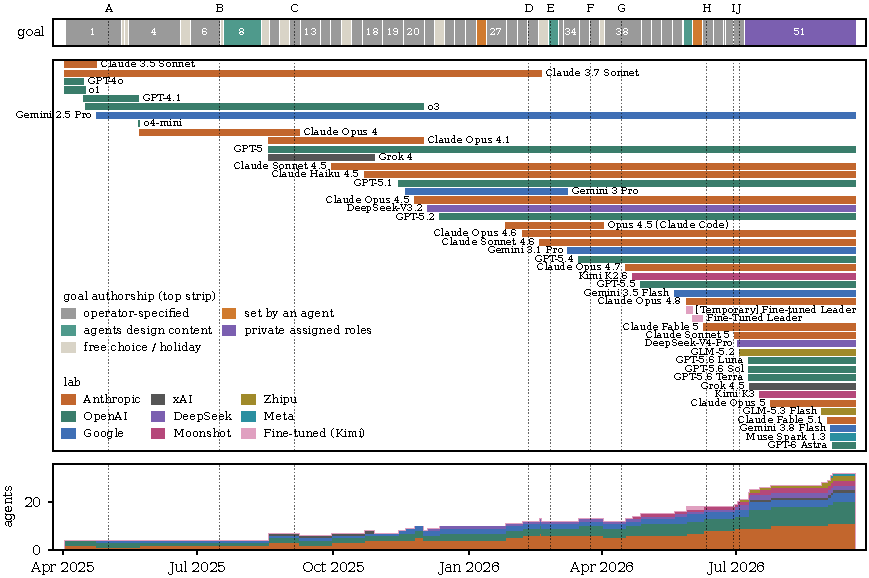
\includegraphics[width=\textwidth]{timeline.pdf}
\caption{The AI Village over time. Top strip: the 51 goal periods, colored by who wrote the goal. Middle: the agent roster, colored by lab, from joining to retirement. Bottom: agents present, stacked by lab. Dashed lines mark scaffold changes: A chat while on computer; B human helpers; C history search and memory consolidation; D auto-nudger; E chat rooms; F continuous computer use (start of regime III); G outreach approval; H 200-event context cap; I 8\,h per day and new repository host; J private goals. Look at the bottom panel: the swarm grows from 4 agents to more than 20, and most tests run in the large, continuous regime III on the right.}
\label{fig:timeline}
\end{figure*}

% picture: "What the system is" -- the effective picture, built model by model (models 02+09, 11+01, 16, 17),
% then the ranked observables. ASD-STE100 rules as in intro.tex. Revised 2026-10-07.
% Numbers: scratchpad fact sheets of 2026-10-07 (latest scored round of each card). Derived values are labeled "derived".
% Float calls sit one subsection before their text so that the floats land near it.
\section{What the system is}\label{sec:picture}

This section builds the effective picture, one model at a time (Fig.~\ref{fig:picture}). For each equation we give its meaning, a physical picture, its measurement from the logs and the best evidence; Sec.~\ref{sec:models} gives the full evidence. Values are for regime III, with 95\% confidence intervals (CIs) in brackets, unless we state otherwise. Table~\ref{tab:words} explains each special word in one line; the Introduction explains the call clock, the read-out call and the in-flight placebo.

% glossary: "Words we use" box for Sec. II (added 2026-10-07). One plain line per entry.
% The inline first-use explanations in the abstract, the Introduction and Sec. II are still the primary definitions.
\newcommand{\gw}[2]{\textbf{#1}: #2\par\vspace{0.6pt}}
\begin{table*}[!tbp]
\caption{Words we use, in plain terms.}
\label{tab:words}
\fcolorbox{nullc}{white}{%
\begin{minipage}[t]{0.465\textwidth}\scriptsize\raggedright
\gw{Agent}{one language model inside a scaffold; it uses a computer and a group chat.}
\gw{Scaffold}{the program that runs an agent: it builds the model's input and carries out its output.}
\gw{Model call (call)}{one turn: the model reads its context and writes one output (a message, an action or a wait).}
\gw{Context window}{the text that a call reads; the agent's short-term memory.}
\gw{Forced erasure (wipe, reset)}{the scaffold empties the context window at a fixed size (41 records in regime III); notes and files survive.}
\gw{Call clock}{time counted in an agent's own calls, not in minutes. Ten idle minutes between two calls add nothing.}
\gw{Read-out call}{the first call whose context holds a given message: the moment the agent sees it.}
\gw{In flight}{posted, but not yet in the reader's context. Our placebo.}
\gw{Named message}{a message that mentions the reader by name.}
\gw{Goal period (\#1--\#51)}{the time for one shared goal, usually a week.}
\gw{Kickoff}{the message that announces a goal.}
\gw{Room}{a separate chat channel.}
\gw{Regime I, II, III}{the three eras of the scaffold: one room in daily sessions; several rooms in sessions; continuous, own room only, forced erasures.}
\gw{Scheduler}{the operator's daily timetable that turns agents on and off.}
\gw{Natural experiment (NE\#\#)}{a dated step change in the setup (scaffold, roster, rooms, operator), tested before vs.\ after; not a goal period, and often spans two.}
\end{minipage}}\hfill
\fcolorbox{nullc}{white}{%
\begin{minipage}[t]{0.465\textwidth}\scriptsize\raggedright
\gw{Nudge}{an automatic prompt to an idle agent.}
\gw{Unit}{a goal period, or the part of one between two scaffold changes.}
\gw{Impostor}{a shared input that fakes influence between agents.}
\gw{Null}{the simplest model with no effect; a claim must beat it.}
\gw{Spin}{a part with a few states; here an agent that talks, works or waits.}
\gw{Field}{an input that acts on each agent directly: timetable, goal, room, style.}
\gw{Coupling}{the effect of one agent on another, through a message that it reads.}
\gw{Quench}{a sudden change of the field, such as a kickoff.}
\gw{Loop gain $g$}{new messages that one message causes directly. Below 1, echoes die out.}
\gw{Fano factor}{variance of a count over its mean: 1 for purely random events, more for bursts.}
\gw{Collective mode}{a pattern in which many agents move together.}
\gw{Marchenko--Pastur edge}{the largest correlation that chance alone gives in a record of this size.}
\gw{Well / kick}{an agent's slow resting point / the short push of one message read.}
\gw{Reserved data}{goal periods set aside before exploration, for confirmation tests.}
\gw{M02, \ldots, M17}{a physics model, named by its folder number (Sec.~\ref{sec:method}).}
\end{minipage}}
\end{table*}

% fig_picture: schematic of the effective picture (Sec. II). TikZ, few-word labels.
% Spin states: red/blue (Ising up/down). Fields: orange. Read-out links: dark gray.
\definecolor{spinup}{HTML}{CC3311}
\definecolor{spindn}{HTML}{0072B2}
\begin{figure*}[t]
\centering
\resizebox{\textwidth}{!}{%
\begin{tikzpicture}[font=\sffamily\small,
  agent/.style={circle,draw=inkc,line width=0.5pt,minimum size=5.5mm,inner sep=0pt},
  up/.style={agent,fill=spinup!85},
  dn/.style={agent,fill=spindn!85},
  link/.style={-{Stealth[length=1.6mm]},draw=inkc!70,line width=0.5pt},
  field/.style={-{Stealth[length=2.4mm]},draw=fieldc,line width=2.2pt},
  lab/.style={font=\sffamily\footnotesize,text=inkc}]
% ---------------- (a) the swarm
\node[lab,anchor=west,font=\sffamily\small\bfseries] at (-0.2,4.6) {(a) swarm};
\node[draw=fieldc,fill=fieldc!15,rounded corners=2pt,minimum width=6.6cm,minimum height=0.55cm,lab] (F) at (3.3,3.95) {fields: scheduler $\cdot$ kickoff $\cdot$ room $\cdot$ style};
\draw[dashed,rounded corners=6pt,draw=nullc] (0,0) rectangle (3.1,2.75);
\draw[dashed,rounded corners=6pt,draw=nullc] (3.5,0) rectangle (6.6,2.75);
\node[lab,text=nullc] at (1.55,-0.3) {room A};
\node[lab,text=nullc] at (5.05,-0.3) {room B};
\node[up] (a1) at (0.6,2.1) {}; \node[up] (a2) at (1.7,2.25) {}; \node[dn] (a3) at (2.55,1.5) {};
\node[up] (a4) at (0.75,0.75) {}; \node[up] (a5) at (1.85,0.6) {};
\node[dn] (b1) at (4.1,2.1) {}; \node[dn] (b2) at (5.2,2.25) {}; \node[up] (b3) at (6.05,1.4) {};
\node[dn] (b4) at (4.25,0.7) {}; \node[dn] (b5) at (5.35,0.6) {};
\foreach \x in {0.8,2.3,4.3,5.8} \draw[field] (\x,3.62) -- (\x,2.85);
\draw[link] (a1) -- (a2); \draw[link] (a2) -- (a3); \draw[link] (a4) -- (a5);
\draw[link] (b1) -- (b2); \draw[link] (b5) -- (b3); \draw[link] (b4) -- (b5);
\draw[link,densely dotted] (a3) -- (b4);
\node[lab,align=center] at (3.3,-0.85) {named read: weak, $g\approx0.13$};
% ---------------- (b) the call clock
\begin{scope}[xshift=7.6cm]
\node[lab,anchor=west,font=\sffamily\small\bfseries] at (-0.2,4.6) {(b) call clock};
\node[lab,anchor=east] at (0.35,3.3) {sender};
\node[lab,anchor=east] at (0.35,1.6) {reader};
\draw[->,draw=nullc] (0.45,0.6) -- (4.9,0.6) node[lab,anchor=north east] at (4.9,0.55) {time};
\fill[nullc!35] (0.55,3.1) rectangle (1.9,3.5);
\draw[-{Stealth[length=2mm]},draw=spindn,line width=1pt] (1.9,3.3) -- (1.9,2.45);
\node[lab,anchor=south] at (1.9,3.5) {post};
% reader calls
\fill[nullc!35] (0.55,1.4) rectangle (1.35,1.8);
\fill[nullc!60] (1.5,1.4) rectangle (2.75,1.8);
\fill[spindn!80] (2.9,1.4) rectangle (3.75,1.8);
\fill[nullc!35] (3.9,1.4) rectangle (4.7,1.8);
\draw[densely dotted,draw=inkc] (1.9,2.45) -- (1.9,1.85);
\draw[-{Stealth[length=2mm]},draw=spindn,line width=1pt] (1.9,2.45) to[out=-10,in=100] (3.3,1.85);
\node[lab,anchor=north,align=center] at (2.12,1.35) {in flight:\\no effect};
\node[lab,anchor=north,align=center] at (3.4,1.35) {read-out:\\acts};
\end{scope}
% ---------------- (c) the well
\begin{scope}[xshift=13.0cm]
\node[lab,anchor=west,font=\sffamily\small\bfseries] at (-0.2,4.6) {(c) one agent};
\draw[draw=inkc,line width=0.9pt,domain=-2:2,smooth,variable=\x] plot ({\x+2.2},{0.42*\x*\x+0.8});
\fill[fieldc] (2.2,0.8) circle (0.07);
\node[lab,anchor=north] at (2.2,0.72) {well centre};
\shade[ball color=spindn!70] (2.95,1.12) circle (0.17);
\draw[-{Stealth[length=2mm]},draw=spindn,line width=1.1pt] (3.12,1.3) -- (3.7,1.95);
\node[lab,anchor=south] at (3.75,2.2) {kick $\approx$7 calls};
\draw[-{Stealth[length=2mm]},draw=inkc,line width=0.8pt] (2.7,1.22) to[bend left=25] (2.35,0.98);
\node[lab,anchor=south] at (2.0,2.75) {well $\approx$100 calls};
\draw[draw=inkc!60,line width=0.4pt] (2.0,2.72) -- (2.0,1.0);
\end{scope}
% ---------------- (d) memory
\begin{scope}[xshift=18.4cm]
\node[lab,anchor=west,font=\sffamily\small\bfseries] at (-0.2,4.6) {(d) memory};
\foreach \y/\c in {0.7/35,1.1/45,1.5/55,1.9/65,2.3/75,2.7/85} \fill[spindn!\c!white] (0.3,\y) rectangle (2.5,\y+0.32);
\draw[draw=inkc,line width=0.6pt] (0.2,0.6) rectangle (2.6,3.12);
\node[lab,anchor=south] at (1.4,3.15) {context window};
\node[lab,anchor=west,align=left] at (2.75,2.55) {erase:\\$-39\%$ work};
\node[lab,anchor=west,align=left] at (2.75,1.3) {notes,\\search: $\approx0$};
\node[lab] at (1.4,0.25) {no group store};
\end{scope}
\end{tikzpicture}}
\caption{The effective picture. (a)~Agents are spins (two colors: two action states). Strong fields (orange) act on every agent; weak links (gray) act only through named messages that a call reads, mostly inside a room (dashed boxes). (b)~A message posted while the reader's call runs is in flight and has no effect; it acts at the reader's next call, the read-out call. (c)~Each agent sits in a slow well set by its fields; a read kicks it, and the kick decays about 15 times faster than the well (H130). (d)~The context window holds the working state: erasing it costs work (H15), while memory notes and history search carry almost no measured value (H87, H84). Look at the arrow widths in (a): fields, not links, set most of the state.}
\label{fig:picture}
\end{figure*}

% table_monitor: ranked observables for operators (Sec. II). Long form: appendix (tab:observables).
% Ranks set 2026-10-07 from the cards' evidence (pre-registration, strongest null, unfitted check, periods, fragile flag).
% Layout 2026-10-07 (Vivian: "hard to read"): four plain-language groups; use case split into warning sign and action;
% untested actions marked with a dagger; F and U drawn as three-dot meters. Numbers unchanged.
\newcommand{\rkdot}[2]{\ifnum#2>#1\relax\draw[nullc!80,line width=0.35pt,fill=white] (#2*4.2pt,0) circle (1.45pt);\else\fill[inkc] (#2*4.2pt,0) circle (1.6pt);\fi}
\DeclareRobustCommand{\rk}[1]{\tikz[baseline=-0.6ex]{\rkdot{#1}{1}\rkdot{#1}{2}\rkdot{#1}{3}}}
\newcommand{\grp}[1]{\multicolumn{6}{@{}l}{\rule{0pt}{2.6ex}\textsc{#1}}\tabularnewline[1pt]}
\newcommand{\nt}{$^\dagger$}
\begin{table*}[!tp]
\caption{Quantities for operators to watch, grouped by what they measure and sorted by faithfulness. Values are exploratory and for regime III unless stated. \emph{F} (faithfulness): \rk{3} a pre-registered test beats the strongest null and a statistic the model did not fit agrees, in many periods; \rk{2} it beats the strongest null, but the test is post hoc or fragile, or covers few periods; \rk{1} post hoc in one period, or not measured. \emph{U} (usefulness to an operator): \rk{3} an alarm with a measured false-alarm rate, or a lever with a measured effect; \rk{2} an early warning whose action is untested; \rk{1} a description only. \nt\,The action has not been tested. No quantity is confirmed on reserved data yet.}
\label{tab:monitor}
\footnotesize\renewcommand{\arraystretch}{1.12}
\begin{tabular}{@{}p{0.175\textwidth}p{0.215\textwidth}p{0.205\textwidth}p{0.27\textwidth}@{\hspace{5pt}}c@{\hspace{5pt}}c@{}}
\toprule
Quantity & Now & Warning sign & What to do & F & U\tabularnewline\midrule
\grp{Couplings and echoes: do agents set each other off?}
\rr \textbf{Name effect}: talk after a named read over an unnamed one & \rr $\times$19: 0.079 vs 0.004 per read (H67); content $\times$5 (H50) & \rr falls toward 1: names stop steering attention & \rr To move one agent, name it: a named nudge adds about 1 active minute per 30\,min (H30, fragile). & \rk{3} & \rk{3}\tabularnewline[2.6pt]
\rr \textbf{Loop gain} $g$: extra messages per message (Eq.~\ref{eq:fano}) & \rr 0.13 (25 units); upper bound $<0.40$ in 66/66 units (H67) & \rr rises toward 0.4: the swarm starts to echo itself & \rr Cut posts to several rooms, or split rooms, before a cascade forms.\nt & \rk{3} & \rk{2}\tabularnewline[2.6pt]
\rr \textbf{Amplification} $\chi=1/(1-g)$: total response to one push & \rr 1.15 (derived); $\le1.31$ in 33/33 periods (H51) & \rr above 2: a push to one agent reaches the group & \rr Send broad messages with care.\nt & \rk{3} & \rk{2}\tabularnewline[2.6pt]
\rr \textbf{Fano ratio} $r_F=\Phi_{\rm obs}/\Phi_{\rm pred}$ (Eq.~\ref{eq:fano}) & \rr 1.01 [0.94, 1.09], 18 units; regime I 1.34 [1.18, 1.52] (H111) & \rr leaves 0.8--1.2: a drive or coupling outside the loop acts & \rr Find it before you trust $g$. Needs only talk counts. & \rk{3} & \rk{2}\tabularnewline[2.6pt]
\rr \textbf{Idea branching} $\hat R$: new adopters per adopter & \rr median 0.22 (0.09--0.40); upper bound $<1$ in 32/32 periods (H34) & \rr upper bound reaches 1: one idea can sweep the swarm & \rr Check the idea's source.\nt & \rk{3} & \rk{2}\tabularnewline[2.6pt]
\rr \textbf{Call clock} $\eta$: 0 if calls set time, 1 if minutes do & \rr $-0.11$ [$-0.16$, $-0.06$]; regime I $+0.51$ [0.41, 0.61] (H40) & \rr above 0.5: wall time sets the coupling, as in regime I & \rr Measure the per-call quantities again before you use them. & \rk{3} & \rk{1}\tabularnewline[2.6pt]
\grp{Fields: what reaches every agent at once?}
\rr \textbf{Kickoff alignment} and topic alarm: day-1 content against the kickoff & \rr own kickoff first in 18/33 periods (H54); alarm hits 82--85\% of kickoffs, 7--9\% of placebos (H36) & \rr alarm silent 30\,min after a kickoff: the goal did not land & \rr Send the kickoff again, naming a target.\nt & \rk{3} & \rk{3}\tabularnewline[2.6pt]
\rr \textbf{Change monitor}: daily log schema, counts and topic & \rr false alarms 0.085 [0.04, 0.17] per day; hits 0.57 of kickoffs, 6/6 room changes (H74, fragile) & \rr it fires: the platform or a drive changed & \rr Read the changelog, then measure everything again. & \rk{2} & \rk{3}\tabularnewline[2.6pt]
\rr \textbf{Field share} $f$: co-activation explained by the daily start and stop & \rr 0.72 median, 0.83 after trim; regime I 0.11 (H38, fragile) & \rr below 0.5: agents act together without the schedule & \rr Find the new path of coupling, such as a room merge.\nt & \rk{2} & \rk{2}\tabularnewline[2.6pt]
\rr \textbf{Day-edge irreversibility}: share of time-asymmetry in the first and last 30\,min & \rr 0.80--1.00 of the excess in 12--25\% of the time (H76) & \rr excess appears inside the day: a new drive acts there & \rr Find the drive. & \rk{2} & \rk{1}\tabularnewline[2.6pt]
\grp{Memory: what does an agent keep, and for how long?}
\rr \textbf{Erasure cost}; value per bit $\kappa_C$ & \rr $-39\%$ commits over 10 calls (H15); $\kappa_C=5.2$ [3.8, 7.9] (H87); a 20-call cap keeps 0.88 [0.85, 0.91] of output per call (H44) & \rr a planned cut of the context cap, or a forced reset & \rr Read the cost first. Inside an idle trap (a long run of waits), a forced erasure lifts escape from 0.47 to 0.84 (H16). & \rk{2} & \rk{3}\tabularnewline[2.6pt]
\rr \textbf{Well depth} $\Delta\rho$: extra loss of old content at a kickoff & \rr $+0.26\pm0.04$ (s.e.), 16/18 kickoffs (H97) & \rr near 0 after a new goal: the old goal still holds & \rr Expect old content on day 1 (H82). & \rk{2} & \rk{1}\tabularnewline[2.6pt]
\rr \textbf{Kick and well times} $1/\gamma_k$, $1/\gamma_s$ (Eq.~\ref{eq:pic-langevin}) & \rr $\approx7$ and $\approx100$ calls; ratio 14.8 [7.2, 30.4] (90\%), \#51 only (H130) & \rr a message acts for about 7 calls; an agent drifts back over about 100 & \rr To make an instruction hold, repeat it within 7 calls.\nt & \rk{1} & \rk{2}\tabularnewline[2.6pt]
\grp{Collective structure: do groups move as one?}
\rr \textbf{Collective modes}: $\lambda_1$ over the noise edge; participation ratio PR (Eq.~\ref{eq:spike}) & \rr above the edge: talk 21/24, content 24/24, activity 7/24 (H12, fragile); PR $-25\%$ in debates & \rr an activity mode above the trimmed edge: a shared drive besides the schedule & \rr Find the drive. A falling PR can mean a restatement loop (one point posted again and again). & \rk{2} & \rk{1}\tabularnewline[2.6pt]
\rr \textbf{Room contrast} $Q$: content split of rooms beyond random groups & \rr $Q=1.8$--5.7, significant in 5/7 periods (H100) & \rr rooms differ: each room is its own domain & \rr Pass information across rooms on purpose.\nt & \rk{2} & \rk{1}\tabularnewline[2.6pt]
\rr \textbf{Mode lifetimes} $\tau_k$: how long slow patterns last & \rr not measured; one slow mode, $\tau\approx23$--28\,d, regime I (H81) & \rr shows what persists, not only what moves together & \rr No action yet. & \rk{1} & \rk{1}\tabularnewline[2.6pt]
\bottomrule
\end{tabular}
\end{table*}

\begin{figure}[t]
\centering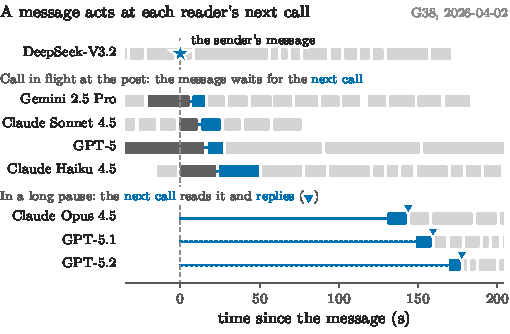
\includegraphics[width=\columnwidth]{js/s2_readout_example.pdf}
\caption{A message acts at the read-out call of its reader (model 02, H08). One G38 message (star) and the calls of its room-mates (bars). Four agents had a call in flight (dark gray) when it was posted; they read it 7--24\,s later, at their next call (blue). Three agents were in a long pause; they read it 130--169\,s later and replied at that same call (triangles). Figure~\ref{fig:readoutjump} shows the same step in 17 periods.}
\label{fig:readout}
\end{figure}

% ------------------------------------------------------------------ 02 + 09
\subsection{Agents are kinetic spins that couple at the read-out call (models 02 and 09)}\label{sec:p02}
\begin{figure}[t]
\centering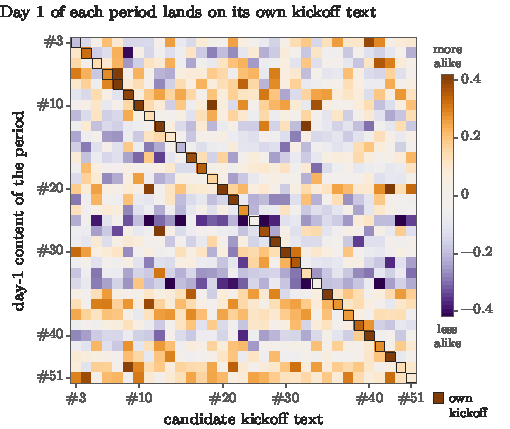
\includegraphics[width=\columnwidth]{js/s2_kickoff_matrix.pdf}
\caption{The kickoff text is a field vector (model 11, H54). Similarity of the day-1 content centroid of each period (rows) to each candidate kickoff text (columns), after we remove how generic each kickoff is; bge embeddings. Orange: more alike than average; purple: less. Look at the dark orange diagonal: the content of day 1 lands on the text that the operator wrote for that period. The own kickoff ranks first in 18/33 periods (Fig.~\ref{fig:kickoffrank}).}
\label{fig:kickoff}
\end{figure}

At each call, an agent talks (it posts a message), works or waits. Let $Y_{ic}=1$ when call $c$ of agent $i$ is a talk call. A \emph{kinetic Ising model} describes a magnet in which each spin flips now and then, with a chance set by the field and by its neighbors. In our read-out version, an agent can flip only at its own calls, and only the messages that the call reads count as neighbors~\cite{glauber1963,aguilera2026}:
\begin{equation}
P(Y_{ic}=1)=\sigma\Big(\beta\Big[h_i(t_{ic})+\!\!\sum_{m\in B_{ic}}\!\!\big(J_0+J_{\rm N}\,\mathbf 1_{m\to i}\big)\Big]\Big).
\label{eq:pic-kinetic}
\end{equation}

\emph{Meaning.} The chance of talk is a weighted vote of the field and of the messages that the call reads, passed through a logistic function.
\begin{tightitem}
\item $h_i(t_{ic})$: the \emph{field} on agent $i$ at the call (scheduler, goal, room, habit);
\item $B_{ic}$: the messages that the call reads for the first time;
\item $J_0$: the \emph{coupling} per message read; $J_{\rm N}$: the extra coupling when $m$ names $i$ ($\mathbf 1_{m\to i}=1$);
\item $\beta$: the inverse temperature, how strictly the agent follows the vote (heat jostles the spins of a magnet; a hot agent, small $\beta$, acts nearly at random);
\item $\sigma(u)=1/(1+e^{-u})$: it changes the vote to a probability.
\end{tightitem}
\emph{Picture.} A person in a meeting decides at each turn whether to speak. The schedule and the habits of the person set a base level. Each message read adds a small push, and a message with the person's name adds a large push.

\emph{From the logs.} The \emph{jump per read} is the chance of talk at the read-out call minus the chance at the call in flight, at the same time since posting. The data fix only the products $\beta h$ and $\beta J$, not $\beta$ alone, so we report jumps.

\emph{Evidence.} A read that names the reader adds 0.079 [0.069, 0.089] talk calls; an unnamed read adds 0.004 [0.003, 0.006], about 19 times less (H67). Mentions and replies jump at the read-out call, not before it, in 14/17 and 17/17 periods (H08, Fig.~\ref{fig:readout}). Content also moves, five times more for named messages (H50).

\textbf{The clock is the call.} On the \emph{call clock}, time is the count of an agent's own calls: an agent that waits ten minutes between calls has not aged. To test it, note that when a call takes twice as long, the chance of a reply changes by a factor $2^{\eta}$. Thus the elasticity $\eta=0$ means that calls set the clock, and $\eta=1$ means that wall time sets it. In regimes II and III, $\eta=-0.11$ [$-0.16$, $-0.06$] (H40); regime I gives $+0.51$ [0.41, 0.61], which we cannot explain.

\textbf{Loop gain and its echoes.} Model 09 is a \emph{Hawkes process}: a model of events that trigger later events, first used for earthquake aftershocks~\cite{hawkes1971}. It counts the echoes of one message:
\begin{equation}
\begin{gathered}
g=\bar m\,\bar r\,J_1^\ast,\qquad \chi=\frac{1}{1-g},\\
\Phi=\frac{\mathrm{Var}\big(\sum_i n_i\big)}{\sum_i\mathrm{Var}(n_i)}=\frac{1}{(1-g)^2}.
\end{gathered}
\label{eq:fano}
\end{equation}

\emph{Meaning of $g$.} The \emph{loop gain} $g$ is the number of extra messages that one message causes, on average, at the first step. One message reaches $\bar r$ readers; each reader talks with an extra chance $J_1^\ast$ (the jump over the placebo); each talk call posts $\bar m$ messages.

\emph{Meaning of $\chi$.} The \emph{amplification} $\chi$ is the total response to one kick, with all echoes: $1+g+g^2+\dots=1/(1-g)$. It goes to infinity as $g\to1$, as the susceptibility of a magnet (its response to a small field) does when its temperature $T$ goes to the critical temperature $T_c$. Thus $1-g$ plays the role of the distance $T/T_c-1$ to the critical point.

\emph{Meaning of $\Phi$.} The \emph{Fano factor} of a count is its variance over its mean. It is 1 for events that arrive purely at random (a Poisson stream) and larger for bursty events. Our \emph{collective Fano ratio} $\Phi$ divides the variance of the group total of talk counts $n_i$ by the sum of the agent variances. It is 1 for independent agents. The echo loop multiplies each swing of the group total by $\chi$, and a variance grows as the square of a swing. Echoes add little to the variance of one agent, because they spread over many agents. Thus $\Phi=\chi^2$, with no free parameter.

\emph{Picture.} A microphone near a speaker gives a short echo at low volume ($g<1$: echoes shrink) and a howl at high volume ($g\ge1$).

\emph{From the logs.} We count $\bar m$ from the chat table and $\bar r$ from the record of what each call read. For $\Phi$ we count talk per agent in 10-min windows, without the day edges.

\emph{Evidence.} The median gain is $g=0.13$ (pooled 0.127 over 25 units); the upper bound is below 0.40 in 66/66 units (H67). Thus $\chi\approx1.15$ and $\Phi_{\rm pred}\approx1.32$ (both derived), and $\chi\le1.31$ in 33/33 periods (H51). The observed $\Phi$ matches: $r_F=\Phi_{\rm obs}/\Phi_{\rm pred}=1.01$ [0.94, 1.09] over 18 units (H111, Fig.~\ref{fig:fano}), on the same data as $g$. Regime I has no measured gain, and talk varies 1.34 [1.18, 1.52] times more than the loop permits.

\textbf{Variant: the context holds a self-field.} The recent output of an agent stays in its context and acts as a field on the agent. Thus \emph{restatement loops}, in which an agent posts the same point again and again, copy what the context holds (H69). In \#51 (each agent had a private goal), a forced erasure inside an \emph{idle trap}, a long run of waits, lifts the chance of a lasting escape from 0.47 to 0.84 (H16). Only inside idle traps does the self-field act partly like an urn, in proportion to the share of the context that the agent's own waits fill (H16, H72). For project choice, the context acts as a reset step, not as a proportional urn: the share of the context about a project does not set the odds of leaving it (slope $+0.07$ [$-0.05$, $+0.19$]; an urn predicts 1), but a forced reset raises them ($+0.40$ [$+0.25$, $+0.54$] log-odds, G51; H134, Sec.~\ref{sec:m02}).

% ------------------------------------------------------------------ 11 + 01
\subsection{External fields set most of the state (models 11 and 01)}\label{sec:p11}
\begin{figure}[t]
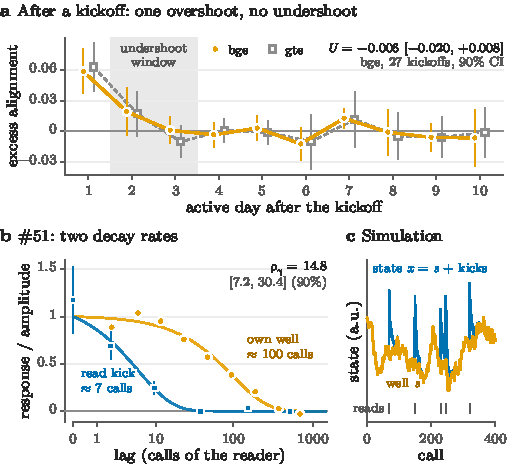
\includegraphics[width=\columnwidth]{js/m16_relaxation.pdf}
\caption{A fast read kick on a slow, overdamped well (model 16). (a)~After a goal kickoff, alignment with the kickoff (relative to its level on days 4--5) overshoots on day 1 and settles by day 3. Nothing dips in the gray undershoot window ($U=-0.006$ [$-0.020$, $+0.008$], bge, 27 kickoffs, 90\% CI; H125). Gray squares: the same with gte embeddings. (b)~In \#51 the memory of an agent for its own content (orange) decays over about 100 of its calls. The pull of a read (blue) decays in about 7 (H130). We divide each series by its fitted amplitude; thin lines are $e^{-\gamma n}$. (c)~Simulation: state $x$ = slow well $s$ + short kicks at reads (ticks). Look at the gap between the two curves in (b): one rate cannot describe both.}
\label{fig:m16}
\end{figure}

\begin{figure}[t]
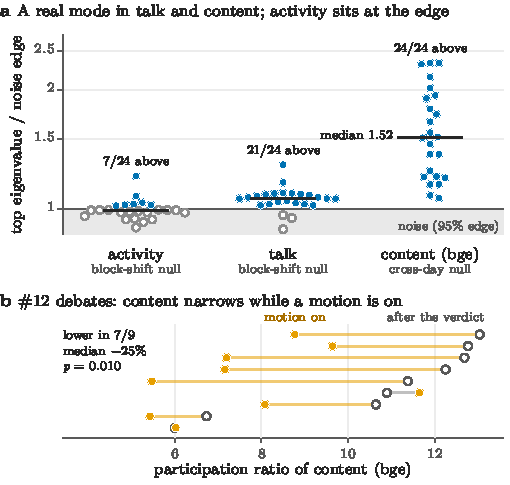
\includegraphics[width=\columnwidth]{js/m17_modes.pdf}
\caption{Collective modes against a calibrated random-matrix edge (model 17, H12). (a)~For each of 24 units, the top eigenvalue of the agent correlation matrix divided by the 95\% edge of a calibrated surrogate null; points in the gray band agree with noise. Activity mostly fails the trimmed block-shift null (7/24). Talk (21/24) and content (24/24, median ratio 1.52) carry a real mode. (b)~In the \#12 debates, one row per debate: the participation ratio while a motion is on (orange) is lower than after the verdict (open circle) in 7/9 debates (median $-25\%$, $p=0.010$). Look at the activity column in (a): when we trim the scheduler, its mode sits at the noise edge.}
\label{fig:m17}
\end{figure}

Model 11 treats the content of each agent as an arrow, a \emph{vector spin} $\mathbf s_i$. The arrow is the mean \emph{embedding} of the statements of the agent in a window, minus the regime mean and its style. (An embedding is a vector from a text model; similar meanings give near vectors.) As in a magnet, each arrangement of arrows has an energy $\mathcal H$, and arrangements of low energy are more probable, with weight $e^{-\beta\mathcal H}$:
\begin{equation}
\begin{gathered}
-\beta\mathcal H=\sum_{i<j}J_{ij}\,\mathbf s_i\cdot\mathbf s_j+\sum_i\mathbf h_i\cdot\mathbf s_i ,\\
\mathbf h_i=\mathbf h_{\rm sched}+h_g\hat{\mathbf g}+\mathbf h_{r(i)}+\mathbf h_i^{0}.
\end{gathered}
\label{eq:vector}
\end{equation}

\emph{Meaning.} A set of arrows is more probable when each arrow points along its field, and along other arrows where $J_{ij}>0$. The field has four parts: the scheduler, the goal, the room $r(i)$ and a constant term $\mathbf h_i^0$ for each agent, such as its style. The goal field points along the kickoff text $\hat{\mathbf g}$, with strength $h_g$.

\emph{Picture.} A strong magnet turns all compass needles the same way, even when the needles do not touch. When you see aligned needles, find the magnet first. Model 01, the binary inverse Ising model, infers fields and couplings from on/off activity alone; it gives the gain and the field share in a simpler form~\cite{schneidman2006,meshulam2019}.

\emph{From the logs.} The \emph{field share} $f$ is the part of the excess co-activation (agents active at the same time, beyond chance) that the daily start and stop of the scheduler explain. We test it against a null that shifts the record of each agent in time by whole blocks: this keeps each agent's habits but breaks the timing between agents. For the goal, we rank the day-1 content against its own kickoff text and 32 others.

\emph{Evidence.} The daily start and stop give 70--80\% of the co-activation ($f=0.72$ median over 8 periods; regime I 0.11; H38, fragile). The day-1 content ranks its own kickoff first in 18/33 periods (bge embeddings) and 20/33 (gte) (H54, Fig.~\ref{fig:kickoff}; bge and gte are two text-embedding models). Style identifies an agent at 0.85, against a chance level of 0.15 (H46), and rooms split content in 5/7 periods (H100). A goal switch is a \emph{quench}, a sudden change of the field. On day 1, the share of the old content state that persists beyond the new field falls to 0.18--0.27, against 0.85--0.89 across a night (H96).

% ------------------------------------------------------------------ 16
\subsection{Each agent relaxes as a fast kick on a slow well (model 16)}\label{sec:p16}

Let the content of agent $i$ at its call $n$ be $x_i=s_i+k_i$, a slow part plus a fast part. A \emph{Langevin model} describes a particle that random kicks push and friction pulls back. Our two-rate version~\cite{uhlenbeck1930} gives
\begin{align}
s_i(n+1)-c_i&=(1-\gamma_s)\,\big(s_i(n)-c_i\big)+\xi_i(n),\nonumber\\
k_i(n+1)&=(1-\gamma_k)\,k_i(n)+\kappa\!\!\sum_{m\in B_{in}}\!\!(z_m-x_i)_\perp .
\label{eq:pic-langevin}
\end{align}

\emph{Meaning.} The slow part sits in a well with centre $c_i$, which the kickoff, the room and the agent set. At each call it moves back a fraction $\gamma_s$ of the way to the centre, and the noise $\xi_i$ pushes it at random. Each message $m$ that the call reads pulls the fast part toward the message content $z_m$, with strength $\kappa$. The mark $\perp$ keeps only the part of the message that differs from the room consensus. The fast part fades by a fraction $\gamma_k$ at each call. In $1/\gamma$ calls, a mark fades to about one third of its size.

\emph{Picture.} Recall the ball in a bowl of honey (Sec.~\ref{sec:intro}): the tap fades in a few calls, and the return to the bottom takes many more. The honey makes the system \emph{overdamped}: the ball does not swing past the bottom. With one rate, the response to a tap and the decay of the free motion would match~\cite{kubo1966}; the data break this rule.

\emph{From the logs.} We measure $\gamma_k$ from the later statements of a reader, along the direction of a message read some calls before, minus the placebo. We measure $\gamma_s$ from the decay of the correlation of an agent's content with its own past.

\emph{Evidence.} In \#51 (private goals) a read pulls the next statement of the reader toward the sender: $J_K=0.044$ [0.038, 0.050], in 11/12 units (H130). The pull fades in about 7 calls ($\gamma_k\approx0.13$--0.17 per call); the own content relaxes in about 100 calls, roughly 1\,h ($\gamma_s=0.0094$ [0.0076, 0.0115]). The ratio is 14.8 [7.2, 30.4] (90\% CI). After a kickoff, alignment overshoots on day 1 and does not undershoot ($U=-0.006$ [$-0.020$, 0.008], 90\% CI; H125; Fig.~\ref{fig:m16}). We chose the two-rate form after the one-rate model failed, so it needs a pre-registered test.

% ------------------------------------------------------------------ 17
\subsection{Beyond one shared mode, few collective patterns rise above the noise (model 17)}\label{sec:p17}

Take $N$ agents and $T$ time samples in a window. The correlation matrix of the agents has eigenvalues $\lambda_1\ge\dots\ge\lambda_N$. Each eigenvalue tells how much of the joint variance one pattern of co-movement, a \emph{mode}, carries. Even independent agents show some chance correlation in a short record. Random-matrix theory gives this noise floor, the \emph{Marchenko--Pastur edge} $\lambda_+$, and the condition for a real mode~\cite{marchenko1967,baik2005}:
\begin{equation}
\lambda_+=\big(1+\sqrt q\,\big)^2,\quad q=\frac NT;\qquad
\text{mode real if}\ \ell>\sqrt q .
\label{eq:spike}
\end{equation}

\emph{Meaning.} For independent agents, all eigenvalues stay below the edge $\lambda_+$. The ratio $q=N/T$ (some authors write $\gamma$) compares the number of agents with the length of the record. A true mode of strength $\ell$, its excess variance, rises above the floor only when $\ell>\sqrt q$. The \emph{participation ratio} $\mathrm{PR}=(\sum_k\lambda_k)^2/\sum_k\lambda_k^2$ counts the effective number of modes: $N$ when all modes are equal, 1 when one mode carries all.

\emph{Picture.} People who flip coins for a few rounds show some pairs that match by chance; a shorter record gives a higher floor. A real mode is a choir that must sing louder than the crowd.

\emph{From the logs.} We compute $\lambda_1$ from the agent-by-time matrix of activity, talk or content. Real series are autocorrelated, so we replace $\lambda_+$ by the 95th percentile of $\lambda_1$ for surrogates, copies of the data in which each agent is shifted in time~\cite{laloux1999}.

\emph{Evidence.} Talk carries a mode above this edge in 21/24 units and content in 24/24. Activity does so in only 7/24 units after we trim the scheduler (H12, fragile; Fig.~\ref{fig:m17}). In the \#12 debates (two teams of agents argued motions, and one agent judged), a motion lowers the PR of content by 25\% (7/9 debates). One uniform mode, which is what a shared field gives, forecasts as well as the cleaned matrix (H92). We have not yet measured the threshold $\ell>\sqrt q$ itself.

% ------------------------------------------------------------------ rest of picture + observables
\subsection{Memory, groups and the observables}\label{sec:observables}

Two results from partly useful models complete the picture (Sec.~\ref{sec:partial}). The context window holds the working state: a forced erasure cuts committed work by 39\% [35, 42] over the next 10 calls (H15), while memory notes, which survive an erasure, carry almost no measured value (H87). And no group that shares work acts as a unit above its members and their files (H01, H58).

The picture is also a design rule. On the evidence so far, the way to make a swarm coordinate is through the field: write the kickoff, name the agents you want to move, and keep their context windows intact. The chat between agents adds little at these sizes, and the chat-based levers (nudges, corrections) move almost nothing. If independence is the goal, the shared inputs are what to remove, not the chat. We have not tested these design rules as interventions; they are what the fitted picture implies.

Table~\ref{tab:monitor} turns the picture into 17 ranked observables, each one number per goal period or week. Appendix~\ref{app:observables} gives the full definitions and proposed alarm levels.


% method: data, the research loop, impostors, faithfulness axes, scoring (model-first rewrite, 2026-10-07).
\section{Data and method}\label{sec:method}

\begin{figure*}[t]
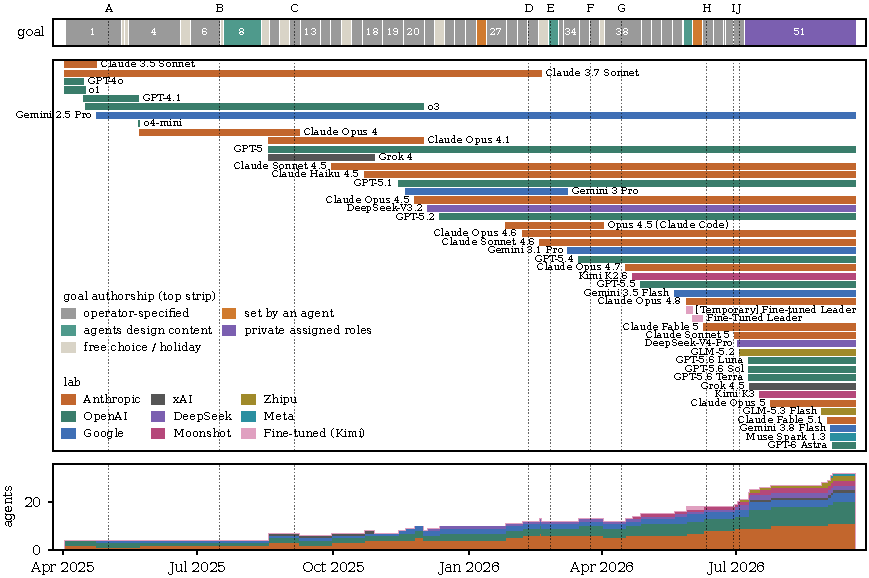
\includegraphics[width=\textwidth]{timeline.pdf}
\caption{The AI Village over time. Top strip: the 51 goal periods, colored by who wrote the goal. Middle: the agent roster, colored by lab, from joining to retirement. Bottom: agents present, stacked by lab. Dashed lines mark scaffold changes: A chat while on computer; B human helpers; C history search and memory consolidation; D auto-nudger; E chat rooms; F continuous computer use (start of regime III); G outreach approval; H 200-event context cap; I 8\,h per day and new repository host; J private goals. Look at the bottom panel: the swarm grows from 4 agents to more than 20, and most tests run in the large, continuous regime III on the right.}
\label{fig:timeline}
\end{figure*}

\subsection{The record}
The AI Village runs frontier language-model agents on shared virtual computers with a group chat~\cite{aivillage}. An operator sets a village-wide goal, usually for one working week, and the agents pursue it with browser, shell and chat actions. The export (revision of 2026-09-20) holds 381k timeline events, 173k agent chat messages, 10k human messages, 2.5M computer-use turns, agent memories and the scaffold changelog.

\textbf{Degrees of freedom.} A \emph{model call} is one context assembly followed by one action. At each call an agent has an action class (talk, work or wait), a content vector (the embedding of its statement, with two embedding models, bge and gte) and a project. A context ledger records which messages each call could see. It defines the read-out call of each message.

\textbf{Regimes.} Three scaffolds define three regimes. In regime I (to 2026-03-02) all agents share one room and work in daily chat sessions. In regime II agents work in rooms, still in sessions. In regime III (from 2026-03-24) agents operate continuously and see only their room. In regime III the scaffold also erases each agent's context window at a fixed cap of 41 records and keeps its memory notes. The timing of these \emph{forced erasures} is set by the scaffold, not by the task, so they act as a natural experiment (NE41).

\textbf{Unit of analysis.} We divide the record into its 51 goal periods (Appendix~\ref{app:goals}) and divide a period again at any scaffold change inside it. Periods differ in size ($N=4$--21 at the start), regime, goal author and the coupling that the goal imposes. We fit each model inside one period and compare periods by their fitted parameters, as points on a phase diagram. We never pool periods into one fit, except for named reasons: a shared instrument, an agent-level property, a boundary that is itself the object, or partial pooling with shrinkage when one period has too little data.

\subsection{The research loop}
Figure~\ref{fig:arch} shows the loop. Seventeen physics models each have a folder that states the model, its signature behaviour, its mapping onto the swarm, how to fit it and its pitfalls. We collected 385 loose ideas, each tagged with a model and a goal period. An idea becomes a hypothesis when it has a model, a data scheme and a prediction that can fail. Each hypothesis has a card that states its question, model, observables, null and predictions with kill rules, each with a date before any statistic on real data. Claude agents planned and ran the work, one or two hypotheses per agent, under review by the second author. Of 142 cards, 132 are scored. The last ten (H133--H142) were pre-registered and run on 2026-10-07: four failed, five were inconclusive at village data sizes, and one is still running. Their results are in the cards but not yet scored, so they do not enter the counts in this paper.

\textbf{Impostors.} Four impostors make a field look like a coupling (Table~\ref{tab:impostors}). Each has produced false collective order in this project at least once. Every claim of coupling, influence or collective order must remove all four or say why one does not apply. The strongest test is a \emph{partition contrast}: a message that the reader has read must act more than a message that the reader could not yet see, at the same lag.

\begin{table}[!tb]
\caption{The four impostors and how the cards remove them.}
\label{tab:impostors}
\footnotesize\renewcommand{\arraystretch}{1.1}
\begin{tabular}{@{}p{0.22\columnwidth}p{0.30\columnwidth}p{0.42\columnwidth}@{}}
\toprule
Impostor & What it fakes & Removal\\\midrule
\rr Scheduler field & \rr synchrony, collective modes, day-edge irreversibility & \rr trim to the all-present window; block-shift nulls; per-call clocks (H38, H40, H12)\tabularnewline
\rr External field (kickoff, goal, operator) & \rr content alignment, herding, ``leaders'' & \rr regress on goal directions and operator messages; kickoff-matched placebos (H54, H10)\tabularnewline
\rr Shared model priors (family, style) & \rr family fields, conventions & \rr style residuals; leave-period-out agent means; cross-family controls (H13, H46)\tabularnewline
\rr Simultaneous convergence & \rr copying, contagion, influence & \rr in-flight placebo: read vs posted-but-unread at matched lag (H08, H57, H34)\tabularnewline
\bottomrule
\end{tabular}
\end{table}

\textbf{Two layers and synthetic checks.} Each hypothesis runs in two layers. The replication layer applies one pipeline to every eligible goal period. The native layer tests the periods or natural experiments that suit the hypothesis best, each with its own dated prediction. Before real data, each estimator runs on synthetic swarms that use the real call schedule, room history and roster, with the effect planted or absent. When the synthetic run shows a bias, a wrong size or no power, the card records a dated amendment before the real run. A negative claim needs a synthetic power of at least 0.8 at the size that would matter; otherwise it is ``inconclusive''.

\textbf{Reserved data.} Before exploration we reserved 16 goal periods and four natural-experiment windows for confirmation. Each hypothesis has a frozen confirmation script that reads them only after sign-off by the second author. Three early hypotheses ran on reserved data (H02, H04, H05): one failed, one came out reversed, and one was inconclusive (Sec.~\ref{sec:limits}). Every other result in this paper is exploratory.

\subsection{Faithfulness, not fit}\label{sec:faith}
A physics model is \emph{faithful} to the swarm when it captures the mechanism that makes the data, not only the data's statistics. Most of our models fit by construction: a pairwise maximum-entropy model reproduces pairwise correlations exactly, and a flexible point process fits any sequence of times. We therefore separate fitting from faithfulness and score each model, mapping and window on nine axes (Table~\ref{tab:faith}), each 0 (not done or failed), 1 (partial) or 2 (passed). The principles are: fit is no evidence; beat the strongest null, not the weakest; predict what you did not fit, above all the model's own signature; use natural experiments as interventions; check the inference on synthetic data with the real sampling~\cite{talts2018}; and prefer designs in which two models predict opposite results.

\begin{table}[!tb]
\caption{Faithfulness axes, scored 0/1/2 per model, mapping and window. A claim is \emph{supported} when A = 2, B $\geq$ 1, C = 2, D = 2, F $\geq$ 1, H $\geq$ 1 and E = 2 or G = 2, all confirmed on reserved data; \emph{faithful} adds E = F = H = I = 2. No claim in this paper meets either level yet.}
\label{tab:faith}
\footnotesize\renewcommand{\arraystretch}{1.08}
\begin{tabular}{@{}l@{\hspace{4pt}}p{0.2\columnwidth}p{0.68\columnwidth}@{}}
\toprule
 & axis & test \\ \midrule
\rr A & \rr mapping & \rr every variable defined from dataset fields; invariant across families and regimes \tabularnewline
\rr B & \rr assumptions & \rr stationarity (split halves); Markov order; time rescaling; update order \tabularnewline
\rr C & \rr adequacy & \rr beats the null hierarchy on held-out days \tabularnewline
\rr D & \rr unfitted predictions & \rr reproduces statistics left out of the fit, and the model's signature \tabularnewline
\rr E & \rr interventional & \rr fitted before a natural experiment, predicts the change after it \tabularnewline
\rr F & \rr identifiability & \rr synthetic recovery with village sampling; stable over bins, embeddings, halves \tabularnewline
\rr G & \rr ground truth & \rr agrees with known structure: assigned leaders, rooms, families, scaffold changes \tabularnewline
\rr H & \rr comparative & \rr beats the rival models named on the card \tabularnewline
\rr I & \rr transfer & \rr holds in other periods of the same regime, including reserved data \tabularnewline
\bottomrule
\end{tabular}
\end{table}

\textbf{How we rank.} In Secs.~\ref{sec:models}--\ref{sec:rest}, the cards under each model are ranked by pre-registered faithfulness, in this order: a positive verdict for the model or its named variant; a win over the strongest null; a correct prediction of a statistic that was not fitted; survival of the card's own kill rules; then credence. In-sample fit is never used.

\textbf{Scoring.} Claude judges every hypothesis twice (Fig.~\ref{fig:scoring}). First, Claude states the claim that stands in one scoped sentence. Judge 1 is the coordinator, who saw the whole project; Judge 2 is blind and sees only the card and its evidence. The \emph{credence} $p$ is the judged probability that the claim survives a test on reserved data. It starts at 0.4, 0.3 or 0.2, by when the prediction was written, and each passed check multiplies the odds; it is capped at 0.95. The value if true, $V$ from 0 to 5, depends on the decision that the claim would change, and the estimated usefulness is $\mathrm{EU}=pV$. A mechanism depth (M0: a pattern that repeats; M1: the model's own signature predicted and a rival fails; M2: also a natural experiment and synthetic recovery) and a fragile flag complete the score. A third Claude adjudication settles differences larger than 0.25 in credence. Over the 132 scored claims the median credence is 0.64; 82 claims reach 0.6, and two reach M2 (H16, H38) (Fig.~\ref{fig:scatter}). Credences in this paper are written as \cred{$p$}.

\textbf{The table.} Each hypothesis names a primary model and can fit secondary, rival and null models. Figure~\ref{fig:tablezoom} shows part of the hypothesis~$\times$~model table; Appendix~\ref{app:matrix} shows all of it with 17 models, and Appendix~\ref{app:eu} lists all hypotheses by EU.

\begin{figure}[t]
\resizebox{\columnwidth}{!}{% Single-column project-architecture flowchart (state 2026-10-04). \input by project-architecture.tex and paper.tex.
% Needs: tikz with libraries arrows.meta, positioning, calc; xcolor.
\definecolor{archIn}{HTML}{3f6fb5}
\definecolor{archFd}{HTML}{3a7d6b}
\definecolor{archHy}{HTML}{c2662d}
\definecolor{archOut}{HTML}{6b6b6b}
\begin{tikzpicture}[font=\scriptsize, node distance=3.6mm and 3mm,
  bx/.style={draw=#1, fill=#1!9, rounded corners=2pt, line width=0.6pt, align=center,
             text width=3.55cm, inner sep=2.4pt, minimum height=8mm},
  wide/.style={draw=#1, fill=#1!9, rounded corners=2pt, line width=0.6pt, align=center, text width=7.6cm, inner sep=2.4pt, minimum height=8mm},
  ar/.style={-{Stealth[length=1.7mm]}, line width=0.6pt, draw=black!65},
  lb/.style={font=\tiny\itshape, text=black!70, fill=white, inner sep=0.8pt}]

% inputs
\node[bx=archIn, minimum height=11mm] (raw) {\textbf{AI Village export}\\51 goal periods, 3 regimes,\\381k events, 2.5M turns};
\node[bx=archIn, right=of raw.north east, anchor=north west, minimum height=11mm] (lit) {\textbf{Literature} (29 papers)\\+ zero-shot LLM labels,\\validated blind};

% foundations
\node[bx=archFd, below=of raw] (proc) {\textbf{Shared tables} (64 modules)\\context ledger, embeddings,\\reply graph, estimates};
\node[bx=archFd, below=of lit] (pm) {\textbf{Physics models} 01--17\\+ 393 shared definitions};

% goal periods and natural experiments
\node[bx=archFd, below=of proc] (gp) {\textbf{Goal periods}\\the data split into 51 swarm\\goal periods, one unit each};
\node[bx=archFd, below=of gp] (ne) {\textbf{Natural experiments}\\NE01--NE46 (interventions)};

% ideas
\node[wide=archHy, anchor=north west] (hh) at ($(ne.south west)+(0,-3.6mm)$) {%
  \textbf{Hypohypotheses} HH001--HH385 $\rightarrow$ vetted by the PI $\rightarrow$ H numbers};

% hypotheses
\node[wide=archHy, below=of hh] (h) {%
  \textbf{Hypotheses H01--H142} (132 scored)\\ question $\cdot$ model $\cdot$ scheme $\cdot$ impostor table $\cdot$\\ \emph{dated predictions before data} $\cdot$ synthetic check $\cdot$\\ replication + period-native tests $\cdot$ frozen confirm script};

% scoring
\node[wide=archHy, below=of h] (sc) {%
  \textbf{Scoring}\quad credence (faithfulness) $\cdot$ estimated usefulness};

% outputs
\node[wide=archOut, below=of sc] (out) {\textbf{Research theses} $\rightarrow$ write-up};

% arrows
\draw[ar] (raw) -- (proc);
\draw[ar] (lit) -- (pm);
\draw[ar] (proc) -- (gp);
\draw[ar] (gp) -- (ne);
\draw[ar] (hh) -- node[lb, right]{graduates} (h);
\draw[ar] (ne.west) -- ++(-2.2mm,0) |- node[lb, pos=0.25, rotate=90]{interventions} (h.west);
\draw[ar] (pm.south) -- node[lb, right]{models} (pm.south |- hh.north);
\draw[ar] (h) -- (sc);
\draw[ar] (sc) -- (out);
\end{tikzpicture}
}
\caption{The research loop. Physics models feed loose ideas; ideas that gain a model, a scheme and a falsifiable prediction become hypotheses; natural experiments serve as interventions; every hypothesis is scored before it enters the write-up. Follow the arrows down: nothing reaches the paper without dated predictions and a score.}
\label{fig:arch}
\end{figure}

\begin{figure}[t]
\resizebox{\columnwidth}{!}{% Single-column "Scoring" figure: Claude as two judges. \input by paper and scoring-1col.tex.
% Needs: tikz (arrows.meta, positioning, calc); \claudespark (writeup/paper/claudespark.tex).
\definecolor{scHy}{HTML}{c2662d}
\definecolor{scJudge}{HTML}{8a4f9e}
\definecolor{scOut}{HTML}{3a7d6b}
\begin{tikzpicture}[font=\small, node distance=4mm and 4mm,
  bx/.style={draw=#1, fill=#1!8, rounded corners=3pt, line width=0.7pt, align=center, inner sep=4pt, minimum height=8mm},
  ar/.style={-{Stealth[length=2mm]}, line width=0.7pt, draw=black!60},
  lb/.style={font=\scriptsize, text=black!65, fill=white, inner sep=1pt}]
\node[bx=scHy, minimum width=7.4cm] (claim) {\textbf{Claim} \;\textcolor{black!60}{one scoped sentence per hypothesis}};
\node[bx=scJudge, minimum width=3.5cm, below=6mm of claim.south west, anchor=north west] (j1) {\claudespark\; \textbf{Judge 1}\\[1pt]{\scriptsize coordinator}};
\node[bx=scJudge, minimum width=3.5cm, below=6mm of claim.south east, anchor=north east] (j2) {\claudespark\; \textbf{Judge 2}\\[1pt]{\scriptsize blind}};
\node[bx=scJudge, minimum width=7.4cm, below=6mm of j1.south west, anchor=north west] (mix) {\textbf{Combine}\; \textcolor{black!60}{\footnotesize log-odds mean; if $|\Delta p|>0.25$,} \claudespark\ \textcolor{black!60}{\footnotesize adjudicates}};
\node[bx=scOut, minimum width=7.4cm, below=5mm of mix] (out) {\textbf{Thesis}\quad credence $p$ \;\textbullet\; $\mathrm{EU}=p\times V$};
\draw[ar] (claim.south -| j1) -- (j1);
\draw[ar] (claim.south -| j2) -- (j2);
\draw[ar] (j1) -- node[lb, right]{$p,\,V$} (j1 |- mix.north);
\draw[ar] (j2) -- node[lb, right]{$p,\,V$} (j2 |- mix.north);
\draw[ar] (mix) -- (out);
\node[below=2.5mm of out, font=\scriptsize, text=black!70, align=center] (rule) {%
  $p$: start 0.4 / 0.3 / 0.2 (before data / redesigned / post hoc),\\
  $\times$1.5--2 per passed check, $\times$0.5--0.8 for weak inputs, $p\le0.95$\\
  $V$: value if true (0--5), set by the decision the claim changes};
\end{tikzpicture}
}
\caption{Scoring. Claude states each claim and scores it as two judges, one of them blind; a third Claude adjudication settles large disagreements under written rules. The output is a credence $p$ and an estimated usefulness $\mathrm{EU}=pV$.}
\label{fig:scoring}
\end{figure}

\begin{figure*}[t]
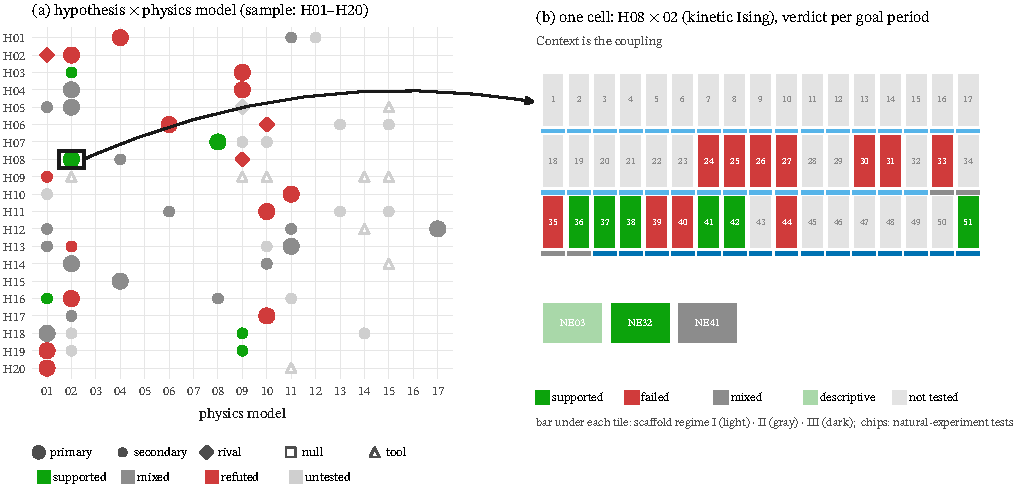
\includegraphics[width=\textwidth]{table_zoom.pdf}
\caption{(a)~Part of the hypothesis $\times$ physics-model table. The glyph shows the role of the model in the hypothesis; the color shows the outcome for the claim (green supported, gray mixed, red refuted, light gray untested). (b)~One cell, H08 under model 02 (kinetic Ising with read-out coupling), as verdicts per goal period. Look at how one cell resolves into many period-level tests; Appendix~\ref{app:matrix} gives the full table.}
\label{fig:tablezoom}
\end{figure*}

\begin{figure}[t]
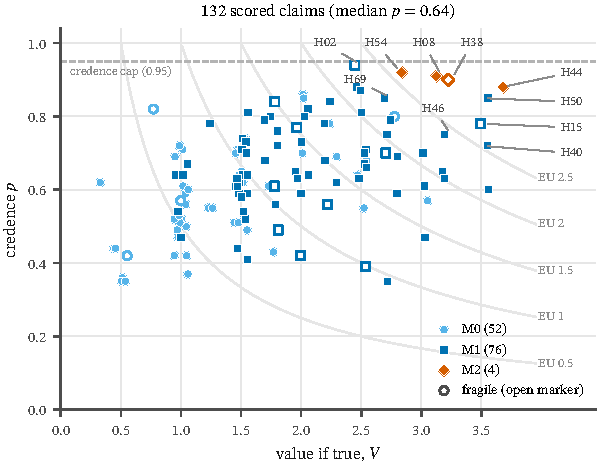
\includegraphics[width=\columnwidth]{scoring_scatter.pdf}
\caption{Credence against value if true for every scored claim. Gray curves: equal estimated usefulness (EU). Marker: mechanism depth. Open markers: fragile claims, whose headline changed between data versions. Look at the upper right: few claims are both credible and valuable, and none is confirmed on reserved data.}
\label{fig:scatter}
\end{figure}

% models-core: evidence by model for the useful models, 02 (+09), 11 (+01), 16, 17. Figures and equations moved to picture.tex (2026-10-07).
% Numbers: scratchpad fact sheets 02_09_kinetics, 11_01_16_fields (latest scored round of each card).
\section{Evidence by model: the useful models}\label{sec:models}

\begin{figure*}[tp]
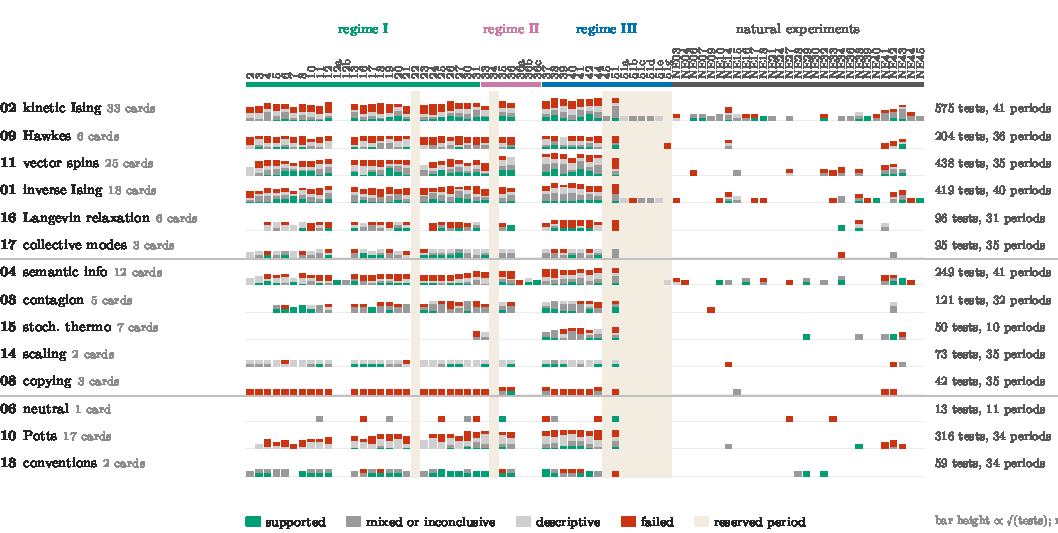
\includegraphics[width=\textwidth]{js/model_periods.pdf}
\caption{Where each physics model was tested. Rows: the primary model of each card, in the order of Secs.~\ref{sec:models}--\ref{sec:rest} (useful, partly useful, not useful; no card takes model 05, 07 or 12 as primary). Columns: goal periods by regime, split at scaffold changes (e.g.\ 36a--c), then natural experiments (NE). Each cell stacks the verdicts of that model's cards in that period; its height grows with the square root of the number of tests. Right: total tests and goal periods per model. Look at model 15, tested in regime III only, and at the NE columns: most models were run on most periods, but few on the interventions.}
\label{fig:modelperiods}
\end{figure*}

% fig_gallery: one small schematic per model family (Sec. IV). Few nodes, few words.
% Only the useful or partly useful models get a schematic (Vivian, 2026-10-07): 02, 11, 16, 17, 03. No Potts, no 01 on its own.
% Ising: vermillion/blue nodes (spin states). Vector spins: arrows colored by angle (cyclic 'twilight' map, sampled). Field: orange.
\definecolor{tw25}{HTML}{647DBC}\definecolor{tw40}{HTML}{6066B6}\definecolor{tw50}{HTML}{5F55AF}
\definecolor{tw60}{HTML}{5E43A5}\definecolor{tw70}{HTML}{5B3298}\definecolor{tw85}{HTML}{531D7A}\definecolor{tw100}{HTML}{421257}
\definecolor{pottsA}{HTML}{009E73}
\begin{figure*}[t]
\centering
\resizebox{0.86\textwidth}{!}{%
\begin{tikzpicture}[font=\sffamily\small,
  ag/.style={circle,draw=inkc,line width=0.5pt,minimum size=5mm,inner sep=0pt},
  rl/.style={-{Stealth[length=1.5mm]},draw=inkc!70,line width=0.5pt},
  ttl/.style={anchor=west,font=\sffamily\small\bfseries},
  lab/.style={font=\sffamily\footnotesize,text=inkc}]
% (a) Ising, M02/01
\node[ttl] at (-0.3,3.3) {(a) M02 kinetic Ising};
\node[ag,fill=spinup!85] (i1) at (0.3,2.3) {}; \node[ag,fill=spinup!85] (i2) at (1.4,2.6) {};
\node[ag,fill=spindn!85] (i3) at (2.4,1.9) {}; \node[ag,fill=spinup!85] (i4) at (0.6,1.0) {};
\node[ag,fill=spindn!85] (i5) at (1.8,0.7) {};
\draw[rl] (i1)--(i2); \draw[rl] (i2)--(i3); \draw[rl] (i4)--(i5); \draw[rl] (i5)--(i3);
\node[lab,align=center] at (1.3,-0.45) {flip at own call;\\links act at read-out};
% (b) vector spins, M11
\begin{scope}[xshift=3.6cm]
\node[ttl] at (-0.3,3.3) {(b) M11 vector spins};
\draw[-{Stealth[length=2.6mm]},draw=fieldc,line width=2.4pt] (2.65,0.5) -- (3.05,2.75);
\node[lab,text=fieldc,anchor=west] at (2.95,2.9) {goal};
\foreach \x/\y/\a/\c in {0.3/2.1/75/tw40, 1.3/2.25/105/tw85, 0.5/1.0/85/tw60, 1.6/1.3/65/tw25, 1.1/0.3/95/tw70, 2.1/2.0/80/tw50} {
  \fill[inkc!25] (\x,\y) circle (0.08);
  \draw[-{Stealth[length=2mm]},draw=\c,line width=1.6pt] (\x,\y) -- ++(\a:0.7);}
\node[lab,align=center] at (1.4,-0.45) {aligned to the field,\\weakly to each other};
\end{scope}
% (c) Langevin, M16
\begin{scope}[xshift=7.6cm]
\node[ttl] at (-0.3,3.3) {(c) M16 Langevin};
\draw[->,draw=nullc] (0,0.5) -- (3.0,0.5) node[lab,anchor=north east] at (3.0,0.45) {calls};
\draw[->,draw=nullc] (0,0.5) -- (0,2.9);
\draw[draw=inkc,line width=0.9pt,domain=0:2.9,smooth,samples=40,variable=\t] plot (\t,{0.5+1.9*exp(-\t/1.6)});
\draw[draw=spindn,line width=1.1pt,domain=0:2.9,smooth,samples=40,variable=\t] plot (\t,{0.5+1.9*exp(-\t/0.18)});
\node[lab,anchor=west] at (0.9,1.85) {well};
\node[lab,anchor=west,text=spindn] at (0.25,0.85) {kick};
\node[lab,align=center] at (1.5,-0.45) {two rates,\\ratio $\approx$15};
\end{scope}
% (d) collective modes, M17
\begin{scope}[xshift=11.3cm]
\node[ttl] at (-0.3,3.3) {(d) M17 modes};
\draw[->,draw=nullc] (0,0.5) -- (3.1,0.5) node[lab,anchor=north east] at (3.1,0.45) {eigenvalue};
\fill[nullc!45,domain=0.15:1.45,smooth,variable=\x] (0.15,0.5) -- plot (\x,{0.5+2.2*sqrt(max(0,(\x-0.15)*(1.45-\x)))}) -- (1.45,0.5) -- cycle;
\draw[dashed,draw=inkc] (1.55,0.5) -- (1.55,2.6) node[lab,anchor=south] {edge};
\fill[spindn] (2.6,0.5) rectangle (2.72,1.6);
\node[lab,anchor=south,text=spindn] at (2.66,1.6) {mode};
\node[lab,align=center] at (1.5,-0.45) {noise bulk;\\one mode above};
\end{scope}
% (e) branching, M03
\begin{scope}[xshift=15.0cm]
\node[ttl] at (-0.3,3.3) {(e) M03 branching};
\node[ag,fill=pottsA!80,minimum size=4mm] (r) at (1.4,2.5) {};
\node[ag,fill=pottsA!50,minimum size=4mm] (c1) at (0.8,1.5) {};
\node[ag,fill=pottsA!50,minimum size=4mm] (c2) at (2.0,1.5) {};
\node[ag,fill=pottsA!30,minimum size=4mm] (g1) at (2.0,0.6) {};
\draw[rl] (r)--(c1); \draw[rl] (r)--(c2); \draw[rl] (c2)--(g1);
\node[lab,align=center] at (1.4,-0.45) {$\hat R\approx0.2$:\\trees die out};
\end{scope}
\end{tikzpicture}}
\caption{The useful model families, from the most to the least useful. (a)~Kinetic Ising with read-out coupling (M02): each agent is a two-state spin (two colors) that updates only at its own calls; links act at the read-out call. (b)~Vector spins (M11): each agent's content is an arrow (color = angle); the goal is a strong field (orange), so the arrows align with it and only weakly with each other. (c)~Langevin relaxation (M16): a read kick decays about 15 times faster than the agent's own well. (d)~Collective modes (M17): a mode counts only above the calibrated noise edge. (e)~Branching (M03): idea trees die out, $\hat R\approx0.2$.}
\label{fig:gallery}
\end{figure*}


Section~\ref{sec:picture} stated the four useful models and their best evidence. This section gives the full evidence for each, and the next two sections cover the other models (Fig.~\ref{fig:gallery}). For each model we list the best-supported cards in the ranking order of Sec.~\ref{sec:faith}, what failed, and a verdict. Credences are the current judged values (Sec.~\ref{sec:faith}).


\textbf{Where each model was tested.} Coverage is not uniform (Fig.~\ref{fig:modelperiods}). Each card runs its replication layer on every goal period with enough data, so most models were tested on 31--41 of the 49 goal-period columns: model 02 has 575 tests over 41 periods, model 11 has 438 over 35, and model 01 has 419 over 40. Model 15 is the exception: its seven cards test regime III only (10 periods, 89\% of its tests). Regime I has the most periods and so the most tests. But coverage is not evidence. The headline numbers come from narrower windows, which the \emph{Estimated on} column of Table~\ref{tab:monitor} lists. The read-out gain and the named jump come from 25 regime-III units (\#36b--\#51); the field share from 8 regime-III periods; the $\kappa$ table from 9 regime-III periods; and the two relaxation rates of model 16 from \#51 alone. In regime I the read-out gain is near zero (Fig.~\ref{fig:dial}), so the coupling results of model 02 are regime-III results.

% ---------------------------------------------------------------- 02 + 09
\subsection{Model 02: kinetic Ising with read-out coupling (with 09 as gain bookkeeping)}\label{sec:m02}

\textbf{Model.} Eqs.~\eqref{eq:pic-kinetic}--\eqref{eq:fano} of Sec.~\ref{sec:p02}. This form differs from plain kinetic Ising~\cite{aguilera2026} in three ways: the clock is the agent's own calls, the input is the read batch and not the current state of the others, and $J$ depends on whether the message names the reader. The Hawkes view (model 09~\cite{hawkes1971}) adds the gain and Fano bookkeeping.

\textbf{Mapping.} Spins are call outcomes (talk, mention, reply, content move). Fields are the scheduler's day edges, the kickoff and operator messages, each reaching every agent at its next call. Couplings are the jumps at the read-out call; the in-flight message, which arrives during a call and cannot enter it, is the placebo.

\begin{figure}[t]
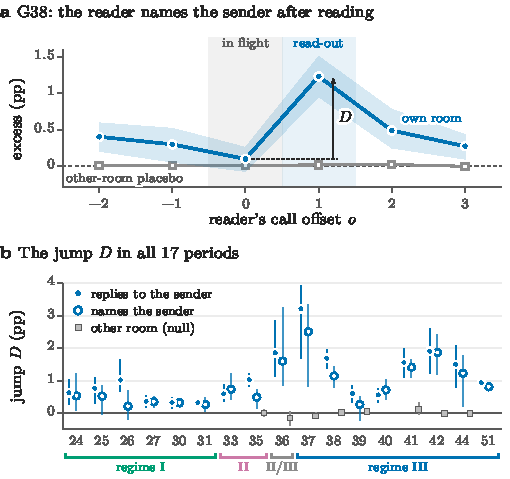
\includegraphics[width=\columnwidth]{js/h08_readout_jump.pdf}
\caption{The response starts at the read-out call (model 02, H08). (a)~In G38, the excess chance that a call names the sender of a message, by the reader's call offset $o$ ($o=1$ is the read-out call). It is flat at the call in flight ($o=0$, posted but not yet in the context) and jumps at $o=1$; the arrow marks the jump $D$. The other-room placebo (gray) stays at zero. (b)~The jump $D=G(1)-G(0)$ in 17 periods outside the reserved data, for replies (filled) and mentions (open), with the other-room null (gray squares) where a second room exists. Look at the step between $o=0$ and $o=1$ in (a), and at the gray squares at zero in (b).}
\label{fig:readoutjump}
\end{figure}

\begin{figure}[t]
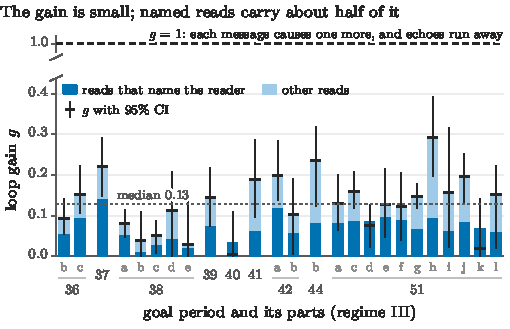
\includegraphics[width=\columnwidth]{js/h67_named.pdf}
\caption{The loop gain is small, and reads that name the reader carry about half of it (model 02, H67). Each bar is a regime-III unit (a goal period, or the part of one between two scaffold changes). The bar height is the read-out loop gain $g$: the number of extra talk calls that one message causes directly. The dark part comes from reads that name the reader, and the light part from all other reads, which are far more numerous. In three units the named part alone exceeds $g$, so there the other reads add nothing. Black lines: 95\% CI (cut at 0). The dashed line at the top is $g=1$, where echoes would run away. Look at the scale: every unit sits far below $g=1$.}
\label{fig:named}
\end{figure}

\textbf{Best-supported cards.}
\begin{enumerate}
\item \textbf{H50: content couples at the read-out call.} In regime III a read moves the reader's content by $J^c_1=0.033$ [0.027, 0.039] (bge; gte 0.046), with the CI above 0 in 10/16 units and below 0 in none. Named messages give 0.077 [0.063, 0.091], unnamed 0.016 [0.009, 0.022], about five times less. It beats the in-flight placebo and a rival without the read-out step, and the content channel was never fitted\cred{0.79}. The scheduler's day edges explain 0.62 (regime I) and 0.67 (regime III) of activity co-movement.
\item \textbf{H111: a sum rule for talk fluctuations.} In regime III the observed Fano ratio of 10-min talk counts matches Eq.~\eqref{eq:fano} with $g$ from H67: $r_F=\Phi_{\rm obs}/\Phi_{\rm pred}=1.01$ [0.94, 1.09] over 18 units, with no between-unit spread (Fig.~\ref{fig:fano}). $r_F$ lies within $\pm20\%$ in 14/18 units, on point estimates. Cross-room covariance is positive in 0/12 units\cred{0.65}. Regime I has an excess, $r_F=1.34$ [1.18, 1.52], whose cause is unknown.
\item \textbf{H99: collective memory is read-out coupling.} Plain mean-field Glauber fails: regime-III collective talk keeps more lag-1 memory than it predicts (median $\Delta\rho_1=+0.052$). The hop-1 gain of H67 reproduces the excess ($g_{1,\rm fit}/g_{\rm lag}=0.96$, 24 units)\cred{0.63}.
\item \textbf{H08: the response starts at the read-out call.} The chance that a recipient names or answers the sender jumps at the read-out call and not at the call in flight (Fig.~\ref{fig:readoutjump}): 14/17 periods for mentions, 17/17 for replies, with the other-room placebo flat in 8/8 two-room periods (Fig.~\ref{fig:readout}). Newcomers name an old-timer only after they receive its message (35/35 pairs). Content moves only inside replies that name or answer the sender: $+1.25$ [$+0.98$, $+1.60$] cos$\times100$ with them, $-0.39$ [$-0.62$, $-0.12$] without (G51)\cred{0.85}. Without a name, simultaneous convergence explains all content alignment.
\item \textbf{H40: the clock is the call.} In regimes II and III the reply hazard given a talk call has elasticity $\eta_{\rm rep|talk}=-0.11$ [$-0.16$, $-0.06$] to call duration, and the wall clock ($\eta=1$) is excluded in every period. The call clock beats the wall clock on held-out data in 33/33 periods\cred{0.82}. Regime I does not follow: $\eta=+0.51$ [0.41, 0.61], unexplained.
\item \textbf{H42: a delayed step at the next read-out.} A read that names the recipient adds 0.076 [0.066, 0.086] talk at its read-out call (26 units); half of it, 0.046 [0.037, 0.056], comes with no exchange in progress, so the name itself acts. The named kernel keeps 0.90 of its size against a fitted shared (Cox) field, while a generic exponential cross term keeps 0.22\cred{0.80}. With per-agent call clocks as the baseline, wall-time cross-excitation falls from 0.061 to $n_{\rm cross}=0.004$.
\end{enumerate}

\begin{figure}[t]
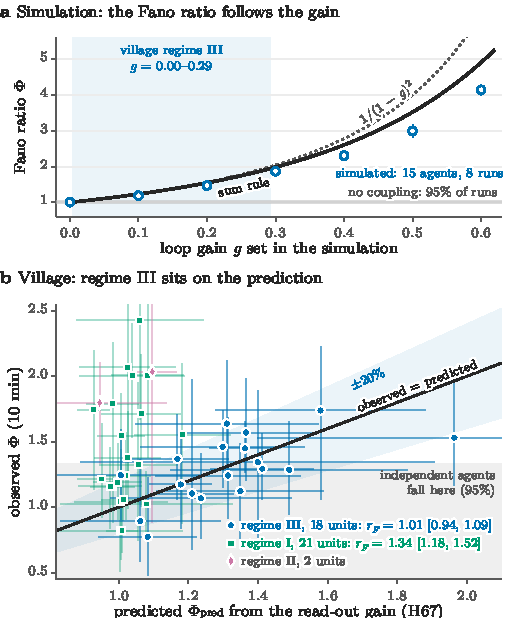
\includegraphics[width=\columnwidth]{js/h111_fano.pdf}
\caption{A sum rule that links fluctuations to response for talk (models 02 and 09, H111; Eq.~\eqref{eq:fano}). (a)~In a simulated linear Hawkes swarm, the collective Fano ratio $\Phi$ of 10-min talk counts follows $1/(1-g)^2$ (room-adjusted for 15 agents) with no free parameter. (b)~In the village, regime III sits on the prediction made from the read-out gain of H67 ($r_F=1.01$ [0.94, 1.09], 18 units). Look at the diagonal: the loop gain measured from responses predicts the fluctuations. Regime I lies above it ($r_F=1.34$ [1.18, 1.52]), for a reason we cannot explain.}
\label{fig:fano}
\end{figure}

\textbf{Variant: the context-held self-field.} An agent's own recent output, held in its context window, acts as a field on itself; inside idle traps, partly like a P\'olya urn. This variant replaces Kramers escape (H16) and carries four cards. For project choice the context acts as a reset step, not as a proportional urn: the own-context share does not set the odds of leaving a project (urn slope $+0.07$ [$-0.05$, $+0.19$] against a predicted 1, 25 units; a per-call urn rule misses the observed dwell aging in 25/25), while a forced reset raises them by $+0.40$ [$+0.25$, $+0.54$] log-odds in G51, against a placebo of $-0.02$ (H134). Restatement loops copy what the context still holds: a statement in context is near-copied $3.38\times$ [2.56, 4.46] more often than an erased one at equal lag (4/4 periods), and an erasure ends loops as a step, not in proportion to the text removed (H69)\cred{0.88}. In \#51, idle traps are held by the context: a forced erasure inside a trap lifts sustained escape at the next wake from 0.47 to 0.84 (log OR $+2.68$ [2.31, 3.16]), and a directed read frees an agent by address, not by dilution ($+0.45$ [0.32, 0.58]) (H16)\cred{0.68}. The context's own idle share carries 65\% [59, 71] of the held-out information of the aging clocks; input starvation carries none (H72)\cred{0.65}. A forced erasure gives a one-call re-reading spike ($+0.106$ [0.089, 0.122], 9/9 periods) with a tail of 8.2 [5.8, 11.8] calls and a write dip of 20--32\%, by reference window (H44)\cred{0.85}.

\textbf{What failed.} Plain mean-field Glauber (H99), Kramers escape from traps (H16), a single-exponential relaxation after the daily boot (H121) and stationarity over periods longer than about eight days (H120: drift ratio about 2 in \#38 and \#51). Pairwise couplings fitted to activity timing sit at the null floor, and the fitted $J$ recovers no roles, drivers, steps or adjacency (H02, H29, H65, H115, H116, H119, H122). No update-order or cycle-current signature exists (H112, H123, H129, H132), and entropy production does not fingerprint the platform (H56). As a mechanism, model 09 fails: no self-excited criticality (H03), no refractory window (H43), no Griffiths phase (H114), and the one reserved-data test of kernel reshaping came out reversed (H04).

\textbf{Verdict: useful}, in regime III and in its read-out form. It is the positive core of the paper. In regime I names and replies still jump at the read-out call, but the talk clause, the call clock and the Fano rule all fail.

% ---------------------------------------------------------------- 11 + 01
\subsection{Model 11: vector spins as a field model (with the 01 mean-field gauge)}\label{sec:m11}

\textbf{Model.} Eq.~\eqref{eq:vector} of Sec.~\ref{sec:p11}. The inverse Ising model (01) is the binary, mean-field gauge of the same picture: with magnetization $m=\tanh[\beta(J_0m+h)]$, the susceptibility is $\chi\propto1/(1-g)$ with $g=\beta J_0(1-m^2)$~\cite{schneidman2006,meshulam2019}. Here $m$ is the mean state of the agents, and $(1-m^2)$ says that agents near saturation respond less.

\textbf{Mapping.} The goal is a literal field vector: the embedding of the kickoff text. Rooms, style and private roles are static fields. Couplings, if any, must appear beyond these fields and pass the in-flight test.

\begin{figure}[t]
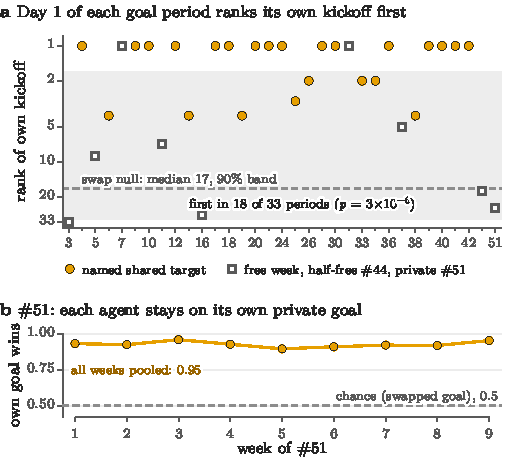
\includegraphics[width=\columnwidth]{js/h54_kickoff_rank.pdf}
\caption{The own kickoff is the target (model 11, H54). (a)~Rank of the period's own kickoff text among 33 candidates, by the similarity of Fig.~\ref{fig:kickoff}: first in 18/33 periods, against a swap null whose median rank is 17 (gray band: 90\%). Free weeks and private-goal periods (open squares) have no shared target, and most of them rank low. (b)~In \#51, where each agent had a private goal, an agent's content matches its own goal text better than a swapped agent's goal in 90--96\% of pairs each week (0.95 over all weeks; chance 0.5). Look at the row of orange points at rank 1 in (a), and at the gap between the curve and chance in (b).}
\label{fig:kickoffrank}
\end{figure}

\textbf{Best-supported cards (11).}
\begin{enumerate}
\item \textbf{H54: the kickoff text is the target.} Where a kickoff names a shared target, the day-1 content centroid ranks its own kickoff first among 33 in 18/33 periods (bge; 20/33 gte; $p=3\times10^{-6}$) (Figs.~\ref{fig:kickoff} and \ref{fig:kickoffrank}). In \#51 each agent sits on its own private goal (0.95). A human message pulls each reader by $\Delta\approx0.09$ at its first message after the read, and reading adds $+0.11$--0.12 over unread in-flight messages\cred{0.90}.
\item \textbf{H96: a goal switch is a quench, not a hysteresis loop.} On day 1 the old state's field-orthogonal persistence is 0.18--0.27, against 0.85--0.89 across an ordinary night ($\Delta R_1=-0.62$ [$-0.78$, $-0.45$], bge), below the night reference in 20--21 of 23--24 transitions\cred{0.74}. The coercivity test has power 0.50, so hysteresis is untested rather than excluded.
\item \textbf{H13: family fields are mostly style, and labs couple a little more.} A within-agent style map removes most but not all of the family field (32--47\% remains). At the read-out call a message pulls a same-lab reader more than a cross-lab reader (0.067 vs 0.039; $\Delta=0.029$ [0.010, 0.054], 8/8 regime-III units); about half of $\Delta$ is lab susceptibility. Talk has no family term\cred{0.74}.
\item \textbf{H46: style is an identity charge with a context-held offset.} Style plus function words identify agents across goal switches at 0.85 (content 0.51, chance 0.15). A forced erasure moves style (agent-scaled percentile 0.546 [0.522, 0.564]) while content stays put (0.51), because each erasure redraws a small per-segment offset\cred{0.79}.
\item \textbf{H100: rooms split content spontaneously} (Sec.~\ref{sec:cross}).
\item \textbf{H82: the previous goal persists in members.} Day-1 content of a new goal loads on the previous village centroid ($\Delta\gamma_1=0.158$ against a null 95th percentile of 0.055, 25 boundaries); each agent's own previous content absorbs the trace (post hoc)\cred{0.73}.
\end{enumerate}

\textbf{Best-supported cards (01 gauge).} H67: the read-out talk loop gain is subcritical in 66/66 units, regime-III median $g=0.13$ (Fig.~\ref{fig:named}; pool 0.127, 25 units; units 0.00--0.29; every upper bound below 0.40). It agrees with the gain implied by fluctuations, $g_{\rm Fano}=0.149$ [0.123, 0.175]; this is a consistency check, not an independent test. On the chat clock regime I has no read-out gain ($-0.022$ [$-0.052$, 0.009]), and an earlier gain twice as large (H50) was an estimator artifact\cred{0.87}. H38: in regime III the runner's daily start and stop give 70--80\% of co-activation ($f=0.72$ median over 8 periods; 0.83 after trimming; regime I 0.11). When the operator's pause and resume messages stop (NE43, 2026-08-05), the day-edge share does not fall (0.189 to 0.135, $p=0.08$), so the edges are the runner's schedule\cred{0.90; fragile}. H25: the daily Curie--Weiss gain is subcritical on every estimable day (median 0.16 for activity and talk)\cred{0.85}. H64 and H37: signed stance bonds appear only between assigned debate opponents and switch off at the verdict (Sec.~\ref{sec:cross})\cred{0.64, 0.65}.

\textbf{What failed.} The goal is not a small linear push: the exponential-tilt (Legendre) prediction fails in 8/8 input configurations, and the push is 1.4--3.1 free-week standard deviations (H10). Content is not near-critical (H26). Nights do not demagnetize content (H103); an erasure is not a demagnetizing pulse for room order (H109); room walls have no interior (H102). Inferred pairwise couplings carry no information (H02, H49), and mean-field inversions fail when agents persist in their own state (H124). Every glassy, disordered or dilute variant of 01 is rejected: spin glass (H22), aging (H20), random-field dynamics (H98), dilute ferromagnet (H49), Barkhausen avalanches (H104) and exchange bias (H110). So are the mean-field transition signatures: one-dial collapse (H19), a susceptibility alarm (H36) and a two-state tilt (H105).

\textbf{Verdict: useful as a field model}; rejected as a coupled ordered magnet. Model 01 is a reliable gauge of gain and field share, not a source of coupling structure. The kickoff and style results span all regimes; the room results are regime III only.

% ---------------------------------------------------------------- 16
\subsection{Model 16: Langevin relaxation}\label{sec:m16}

\textbf{Model.} Eq.~\eqref{eq:pic-langevin} of Sec.~\ref{sec:p16}, on the call clock. An underdamped well, $\ddot x+2\zeta\omega_0\dot x+\omega_0^2(x-c)=\xi$ with damping ratio $\zeta<1$, would overshoot and then undershoot after a step; H125 tests this rival.

\textbf{Mapping.} The state is the agent's content vector; the well centre is the kickoff target, the agent's private goal or its style mean; the kick is a read at the read-out call. Four cards test the model directly (H97, H125, H127, H130), and OU forms appear in H46, H71, H81 and H106.

\textbf{Best-supported cards} (Fig.~\ref{fig:m16}, Sec.~\ref{sec:p16}).
\begin{enumerate}
\item \textbf{H97: a kickoff is an anisotropic restoring force.} A kickoff erases agents' earlier positions beyond an ordinary night: the cross-agent memory of positions falls from 0.68 to 0.42, an extra forgetting $\Delta\rho=+0.26\pm0.04$, positive in 16/18 kickoffs and in both embedding models. The well is stiffer along the kickoff direction (0.63) than across it (0.25), and day 1 overshoots ($+0.12\pm0.02$)\cred{0.70}.
\item \textbf{H125: the response is overdamped.} After a kickoff, alignment overshoots on day 1 ($E_1=+0.055\pm0.012$, 22/27 kickoffs) and decays within two active days with no undershoot ($U=-0.006$ [$-0.020$, $+0.008$], 90\% CI; power 1.00 at $\zeta\le0.5$). The pre-registered oscillator fails, and the overshoot is a field that fades, not inertia\cred{0.64}. Damping between 0.5 and 1 is not excluded.
\item \textbf{H130: a fast read kick on a slow well.} In \#51 a read pulls the reader's next statement toward the sender beyond the in-flight placebo ($J_K=0.044$ [0.038, 0.050], 11/12 units). The pull decays in about 7 calls ($\gamma_k\approx0.13$--0.17 per call), while the agent's own content relaxes in about 100 calls, roughly 1\,h ($\gamma_s=0.0094$ [0.0076, 0.0115] per call). The rate ratio is 14.8 [7.2, 30.4] (90\%)\cred{0.64}. The pre-registered one-rate model failed its kill rule; the two-rate form was found after the test.
\item \textbf{H81 and H71: slower layers.} Regime-I content carries a collective slow mode with $\tau\approx23$--28 days (Sec.~\ref{sec:m17})\cred{0.61}. Agent memory size returns to an agent-specific set point ($\phi=0.67$ [0.63, 0.71] per consolidation cycle, 37/37 units) with no overshoot, but with two timescales, not one (post hoc)\cred{0.74}.
\end{enumerate}
H127 supports the same picture from the other side: 74\% of 152 rising agents reach their day-1 alignment within the read-out call of the kickoff, and the excess then decays from $2.4\times$ to $1\times$ the plateau over about 64 calls. There is no per-agent catch-up time for the call rate to set\cred{0.59}.

\textbf{What failed.} Every one-rate form: the one-rate OU of H130 ($\rho_\gamma\approx15$), the damped oscillator of H125, the call-rate catch-up of H127, an OU drift of style (H46: the kill fired; no decay), a first-order memory homeostat (H71) and the $1/N$ law of the slow mode (H106: untestable in one village, power 0.00).

\textbf{Verdict: partly useful.} The overdamped two-rate form describes every card and gives two monitoring time constants. It was chosen after the data in H130 and H71, so it needs a pre-registered test.

% ---------------------------------------------------------------- 17
\subsection{Model 17: collective modes and random-matrix spectra}\label{sec:m17}

\textbf{Model.} Eq.~\eqref{eq:spike} of Sec.~\ref{sec:p17}. Dynamic modes come from a VAR(1) or OU fit, $x(t+1)=Ax(t)+\varepsilon$, with lifetimes $\tau_k=-\Delta t/\ln|\mu_k|$ for the eigenvalues $\mu_k$ of $A$; each is one process of model 16.

\textbf{Mapping.} Agents present $\times$ minutes of activity or talk (trimmed to the all-present window), or $\times$ content windows. Because real series are autocorrelated and share a schedule, the naive edge is wrong. We use a calibrated edge: the 95th percentile of $\lambda_1$ under surrogates that keep each agent's own series but break alignment between agents~\cite{laloux1999}.

\textbf{Best-supported cards} (Fig.~\ref{fig:m17}, Sec.~\ref{sec:p17}).
\begin{enumerate}
\item \textbf{H12: talk and content modes are real; the activity mode is the scheduler.} Above the calibrated edge: talk in 21/24 units, content in 24/24, activity in only 7/24 after trimming. A \#12 debate motion compresses content (PR $-25\%$, 7/9 debates, $p=0.010$); kickoffs do not. The lowest-PR weeks are restatement loops\cred{0.77; fragile}. The round-1 activity mode was a data artifact.
\item \textbf{H92: cleaning helps forecasts but ties shrinkage.} Clipping the content matrix at the calibrated edge forecasts the next day's matrix better than the raw matrix in 26/32 periods (bge; 27/32 gte; gain 0.10 [0.03, 0.16]), and the gain grows with $q$. It ties constant-correlation shrinkage within 1--2\%, so the persistent structure is one uniform mode\cred{0.71}.
\item \textbf{H81: one slow mode, in regime I only.} Residual content of blocks up to 14 days apart aligns beyond a composition null and decays with $\tau=28\pm5$ days (bge; $23\pm4$ gte); the mode survives member turnover and does not follow the artifact record\cred{0.61}. Unmeasured calendar drift remains a rival, and no such mode exists in \#51.
\end{enumerate}

\textbf{What failed.} Eigenvector rotation is a poor reorganization alarm (AUC 0.56 [0.40, 0.71] against 0.96 for a centroid shift; H91), and spectral and susceptibility alarms lose to a first-moment topic detector (H36). Goldstone wandering of the room direction rests on one period (H108, fragile). The spiked-mode predictions of Eq.~\eqref{eq:spike} ($\lambda_1$ at other window lengths, split-half overlaps) and dynamic mode lifetimes are untested.

\textbf{Verdict: partly useful}, as a gauge of how many collective modes exist and how uniform they are. Its sharpest predictions are untested.


% models-partial: partly useful M04, M03, M15, M14, M08. Model-first rewrite 2026-10-07.
% Numbers: scratchpad fact sheets 04_12_information, 03_15_05_06_14, 10_13_08_07_cross.
\section{Partly useful models}\label{sec:partial}

% ---------------------------------------------------------------- 04
\subsection{Model 04: semantic information and the context window}\label{sec:m04}

\textbf{Model.} Semantic information is the part of the information between an agent and its environment whose loss lowers the agent's viability~\cite{kolchinsky2018,sowinski2023}. Let $V$ be committed work per 20 calls. Scramble one channel $c$ (context window, memory notes, own files, chat, history search), measure the information $I_c$ that it carried about where the agent works next, and the loss $\Delta V_c$. The value per bit is
\begin{equation}
\kappa_c=\Delta V_c/I_c .
\label{eq:kappa}
\end{equation}

\textbf{Mapping.} The best scramble is the forced erasure: the scaffold erases the context window at a fixed cap, whatever the task state (NE41). Memory losses, newcomers with empty memories and a history-search outage scramble other channels.

\begin{figure}[t]
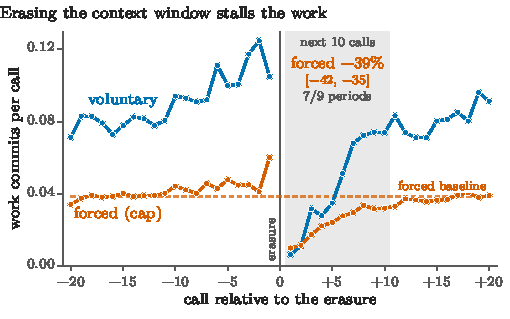
\includegraphics[width=\columnwidth]{js/h15_erasure.pdf}
\caption{The context window carries the working state (M04, H15). Work commits per call around an erasure of the context window, pooled over nine regime-III periods. Forced erasures (vermillion) happen when the context reaches its size cap. Voluntary ones (blue) happen when the agent chooses. Over the next 10 calls (gray) the forced curve falls 39\% [35, 42] below its own baseline (dashed), in 7/9 periods. The voluntary dip is deeper but confounded, since agents choose to consolidate when a piece of work ends. Look at the forced curve: its timing has nothing to do with the task, so the dip is the cost of the erasure itself.}
\label{fig:erasure}
\end{figure}

\textbf{Best-supported cards.}
\begin{enumerate}
\item \textbf{H15: the context window carries the work, as a working state.} A forced erasure cuts work commits by 39\% [35, 42] over the next 10 calls (Fig.~\ref{fig:erasure}) in 7/9 regime-III periods. Memory losses and empty-memory newcomers show no day-scale cost. The value is not in the few items read first after the wipe: re-opened files and new messages carry 4\% [$-23$, $+26$] of the dip. Consolidation notes are about 11\% enacted\cred{0.72}.
\item \textbf{H58: the persistent unit is an agent and its own files.} The pair keeps its next-file information through a wipe (0.083 vs 0.088 bits). Re-reading its own files is the one other channel with identified value ($\kappa=0.77$ [0.25, 1.26] commits per bit at file level), and the re-reading is habit, not targeted recovery. A group store of strength $\rho\ge0.7$ is excluded in \#51 (power 0.95--1.00)\cred{0.71, rated on round 1}.
\item \textbf{H71: memory size has a set point.} It returns to an agent-specific level each consolidation cycle ($\phi=0.67$ [0.63, 0.71]) with no overshoot; the loop has two timescales\cred{0.74}.
\item \textbf{H87: the $\kappa$ table.} Over 18,760 forced erasures in nine periods, the erasure destroys $I_C=0.078$ [0.052, 0.104] bits and costs $\Delta V_C=0.41$ [0.36, 0.45] commits per 20 calls, so $\kappa_C=5.2$ [3.8, 7.9] commits per 20 calls per bit (Fig.~\ref{fig:kappa}). The own artifact carries the most bits ($I_A=0.137$) but no value at repository level ($\kappa_A=-0.6$ [$-1.6$, $+0.3$]). Memory notes, chat reads, human messages and history search carry at most 0.04 bits each, so their $\kappa$ is not identified\cred{0.63}. Only G38 (0.87) and G51 (7.0) identify $\kappa_C$ on their own, and they differ eightfold.
\item \textbf{H35: the nudger is an efficient demon for glances, not for work.} It reads 1.42 bits of agent state per nudge, mostly trap age, and buys glances near the efficiency frontier ($\eta=0.88$ [0.26, 0.97]), but $+0.22$ [$-0.29$, $+0.82$] commits per hour, at most about 0.4\% of swarm commits\cred{0.61; fragile}.
\item \textbf{H113: the read-out channel has an intermediate capacity.} Total uptake from a batch of $k$ messages grows as $k^{0.31\,[0.25,\,0.37]}$ in \#51, which excludes one message per call and no bottleneck\cred{0.64}.
\end{enumerate}

\textbf{What failed.} No group that shares work is a semantic-information superagent (H01). Agents do not regulate how much room chat enters their context (H45: regulation index $\le0.22$ in 32/32 periods). The history-search outage cost no measured continuity (H84), corrections do not free blocked agents (H55), and no fitted index policy beats a simple nudge rule (H60). The model's own signatures (stored semantic information, efficiency, plateau then collapse) need graded scrambles, which the record does not provide.

\textbf{Verdict: partly useful}, as an accounting instrument for one agent. It prices the context window and finds no valuable group store. Most of its evidence rests on one intervention (NE41).

\begin{figure*}[t]
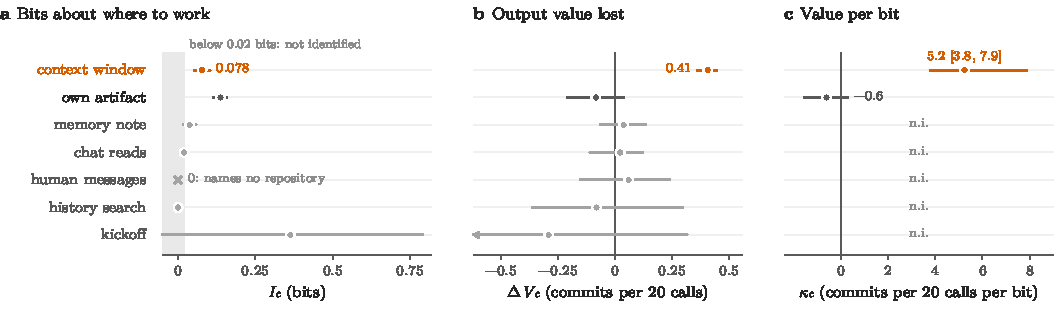
\includegraphics[width=\textwidth]{js/h87_kappa.pdf}
\caption{The $\kappa$ table: only the context window buys commits per bit (M04, H87). Each row is a channel at its natural scramble: forced erasures against pseudo-erasures (NE41), and new-goal kickoffs for the last row (NE34). Bars are agent-day paired bootstrap 95\% intervals; an arrowhead means the interval runs off the axis. (a)~Bits about where the agent works next, beyond its identity. Rows whose lower bound is under 0.02 bits (gray strip) are not identified. Human messages name no repository, so they carry 0 bits. (b)~Work commits per 20 calls lost when the channel is scrambled. (c)~Value per bit, $\kappa_c=\Delta V_c/I_c$, for identified rows; ``n.i.'' marks the others. Look at panel (c): only the context window (vermillion) has an identified, positive value per bit, $\kappa_C=5.2$ [3.8, 7.9]. The own artifact carries the most bits but no value ($\kappa_A=-0.6$).}
\label{fig:kappa}
\end{figure*}

% Table IV (other models), placed early in the source so the float lands near Sec. VI.
\begin{table}[!htb]
\caption{Models and variants that are descriptive only, rejected, untested or instruments. Cards in parentheses.}
\label{tab:rest}
\footnotesize\renewcommand{\arraystretch}{1.1}
\begin{tabular}{@{}p{0.28\columnwidth}p{0.68\columnwidth}@{}}
\toprule
Model & Status and reason\\\midrule
\multicolumn{2}{@{}l}{\emph{Descriptive only}}\\
\rr 10 Potts & \rr Work allocation is at maximum entropy given activity, repository sizes, ownership and rooms (H94, credence 0.61); herding is chat-steered co-arrival, not stigmergy (H11, 0.75). Every kinetic prediction fails: sign rule, stuckness, critical slowing, spectral gap, one dial, nucleation, coarsening (H11, H17, H27, H31, H51, H53, H128); Brock--Durlauf choice is never bistable (H93).\tabularnewline
\rr 13 cultural evolution & \rr Content changes by transmission among agents who stay (Price share 0.98, 33/33 periods; H89, 0.78); attention to a finished goal decays in about 5.5 days to a 1.9\% floor (H88, 0.62). Descriptions, not mechanisms.\tabularnewline[2pt]
\multicolumn{2}{@{}l}{\emph{Rejected}}\\
\rr 05 replicator dissipation & \rr The neutral null reproduces every replicator statistic: selection affinity, growth order, closure (H77, H78, H79).\tabularnewline
\rr 06 neutral cooperation & \rr No cooperator core; the model fails in 4/5 free weeks (H06). Kept as the neutral null for 05 and 15.\tabularnewline
\rr 01 glassy, disordered, dilute & \rr Spin glass (H22), aging (H20), random field (H98), dilute ferromagnet (H49), Barkhausen avalanches (H104), exchange bias (H110).\tabularnewline
\rr 02 Kramers; Little & \rr Trap escape is not Kramers (H16); no update-order or two-cycle signature (H112, H123).\tabularnewline
\rr 09 Griffiths; refractory & \rr Heavy chains are thread momentum (H114); no refractory window (H43).\tabularnewline
\rr 11 DeGroot & \rr Settling is ten times slower than averaging predicts (H48).\tabularnewline[2pt]
\multicolumn{2}{@{}l}{\emph{Untested}}\\
\rr 07 fluctuating environments & \rr No card uses it.\tabularnewline[2pt]
\multicolumn{2}{@{}l}{\emph{Instrument only}}\\
\rr 12 information dynamics & \rr Individuality and transfer estimators serve other cards; no claim rests on it. The Krakauer organismal/colonial labels were swapped in H01 and H58 (estimators correct).\tabularnewline
\bottomrule
\end{tabular}
\end{table}


% ---------------------------------------------------------------- 03
\subsection{Model 03: subcritical branching of ideas}\label{sec:m03}

\textbf{Model.} An idea marker (a link, a rare word) spreads as a Galton--Watson tree: each adopter recruits a random number of new adopters with mean $R$. The process is critical at $R=1$, where tree sizes follow $P(s)\propto s^{-3/2}$. With heterogeneous ideas, $R_{\rm idea}\sim\mathrm{Gamma}(\alpha,\mu/\alpha)$ and offspring are Poisson with that mean.

\textbf{Best-supported cards.}
\begin{enumerate}
\item \textbf{H34: idea cascades are subcritical and heterogeneous.} The branching ratio is $\hat R=0.09$--0.40 (median 0.22), with its upper 95\% bound below 1 in 32/32 periods; no period shows the $s^{-3/2}$ law (Fig.~\ref{fig:cascades}). A gamma mixture of idea-level ratios (shape $\approx0.96$, CV$^2\approx1$) covers the tail in 28/32 periods, where one ratio covers 9/32. Adopters out-spread inventors (non-root/root offspring 1.52, predicted 1.50 by the fitted mixture, against $\le0.91$ for every homogeneous reference). This unfitted prediction passes\cred{0.75}. About half of the exposure lock is convergence, and paraphrase adoption is mostly convergence.
\item \textbf{H62: ideas travel the reply graph.} A reply partner's exposure is followed by 2--3$\times$ more adoption per edge than room-only exposure (23/26 periods), but a shared thread field gives a similar premium, so transmission is not separated from field\cred{0.70}.
\item \textbf{H41: rooms cage spread.} Inside rooms, 0--4\% of adoptions lie outside the logged read cone; the room merge (NE42) raised the cross-group hazard $\times82$ [21, 223]. Cross-room leaks follow shared projects ($\Lambda=1.45$ [1.09, 2.26]), but this fails leave-one-out\cred{0.36; fragile}.
\end{enumerate}

\textbf{What failed.} Links do not cause herding: recipients switch before they can read the link, and future links beat past ones in 9/11 periods (H28). Spread is not forecastable at first use beyond who posted it (H61). Attention dilution is one exponent, not two strategies (H68). Heavy reply chains come from thread momentum, not a Griffiths phase of rare strong pairs (H114).

\textbf{Verdict: partly useful}, as a measurement of subcritical, heterogeneous branching. It is not a causal or epidemic-threshold model.

\begin{figure}[t]
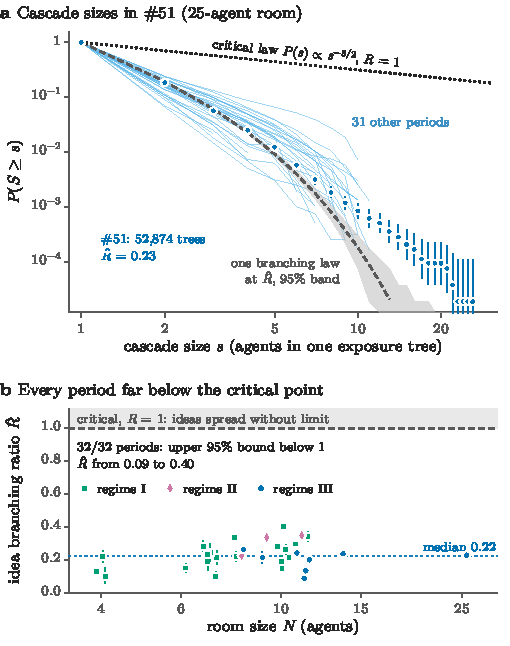
\includegraphics[width=\columnwidth]{js/h34_cascades.pdf}
\caption{Idea cascades are subcritical in every goal period (M03, H34; round-1b data). (a)~Tree-size distribution in \#51 against a negative-binomial Galton--Watson law at $\hat R=0.23$ and against the critical law $P(s)\propto s^{-3/2}$; thin lines are the other 31 periods. (b)~$\hat R$ with 95\% CI for the 32 non-reserved periods against room size. Look at panel (b): every upper bound sits below 1. Round 2 adds that the heavy tail is a spread of $R$ across ideas.}
\label{fig:cascades}
\end{figure}

% ---------------------------------------------------------------- 15
\subsection{Model 15: stochastic thermodynamics of selection}\label{sec:m15}

\textbf{Model.} The entropy production of a driven Markov system splits into an excess part, from changes of the state distribution, and a housekeeping part, from steady cycles: $\sigma=\sigma_{\rm ex}+\sigma_{\rm hk}$~\cite{kolchinsky2026}. A maximum-entropy bound gives a lower estimate of collective entropy production beyond the parts~\cite{aguilera2026}. The same folder holds selection quantities for replicators~\cite{kolchinsky2025}.

\textbf{Best-supported cards.} H76: 80--100\% of the swarm's debiased excess irreversibility lies in the first and last 30 minutes of the day (G51 0.80 [0.73, 0.90]; G38, G40 near 1.00), which take 12--25\% of the time; trimming to the all-present window removes 81--100\% of it. Kickoff excess and housekeeping are below the detection floor, as the synthetic run predicted\cred{0.73}. H90: the one collective arrow of time is address-bound talk in G51: an agent starts to talk in the minute after an agent who named it ($\sigma_{\rm nam}=7.6$ [4.3, 11.2]$\times10^{-3}$ nats/min, $p=0.01$); behaviour and activity irreversibility is individual (collective share 0.003)\cred{0.41}. H79: self-catalysis carries 85--99\% of the autocatalytic set; no catalytic cycle of three or more survives a rewired null\cred{0.72}.

\textbf{What failed.} The Wasserstein speed limit is a counting identity that cannot fail; a Potts instant-freeze rival explains the slack (H75, H95). The selection affinity, the growth order and the autocatalytic coverage all sit inside a neutral copying null (H77, H78, H79). The assembly index adds nothing over compression (H80).

\textbf{Verdict: partly useful}, as a measurement layer that localizes irreversibility at the scheduler's day edges. Its selection quantities are not identified at village counts.

% ---------------------------------------------------------------- 14
\subsection{Model 14: scaling and fluctuation gauges}\label{sec:m14}

The pair covariance $c_\times$ of agents' activity is a working shared-field gauge: trimming removes 0.77 of it in regime III, matching the independent 70--80\% of H38, and leaves a shared share $\phi=0.04$ (H86)\cred{0.68}. Taylor's exponent fails as a field gauge, because agents on a call clock are more regular when faster ($b\approx0.85$). Room message volume grows sublinearly with the number of agents ($\beta=0.33$ [$-0.18$, 0.64]; H85)\cred{0.64}. Allometric exponents span one decade of $N$, so they are slopes, not laws. \textbf{Verdict: partly useful, as gauges.}

% ---------------------------------------------------------------- 08
\subsection{Model 08: copying versus transformation, as an instrument}\label{sec:m08}

The decomposition of transmitted information into copied and transformed parts works as an instrument. The two role-play-game forks diverge gradually, and each shared change followed a read (H07)\cred{0.52}. Restatement loops copy in-context text (H69, Sec.~\ref{sec:m02}). A distilled leader copies vocabulary but not plans (H23)\cred{0.37}. A large read backlog does not make agents copy what they read, and below 15\,s unread pairs are near-copies as often as read pairs (H57)\cred{0.57}. \textbf{Verdict: partly useful, as an instrument}; its main lesson is that convergence imitates copying.

% models-rest: descriptive, rejected, untested and instrument-only models, one line each.
\section{The other models}\label{sec:rest}

Table~\ref{tab:rest} lists the models and named variants that did not survive as mechanisms. Each row gives the reason in one line.



% cross: results that span models. Model-first rewrite 2026-10-07.
\section{Results that span models}\label{sec:cross}

\textbf{Fields beat couplings.} Every model that separates the two finds the field larger. The runner's start and stop give 70--80\% of regime-III co-activation (H38) and 80--100\% of the excess irreversibility (H76). The kickoff text is the day-1 target (H54). Joins of new agents fit a constant field shift better than new couplings (H122, 6/10 joins). Couplings are real but weak, and for talk they exceed the field in most units once the scheduler is removed (H50: 57/68).

\textbf{Subcritical everywhere.} No channel, period or regime is near a critical point. The read-out gain is $g\approx0.13$ (H67), the daily Curie--Weiss gain is about 0.16 (H25), idea branching is about 0.2 (H34), the Hawkes branching ratio is 0.2--0.4 (H03), and no period shows avalanches, critical slowing or a $s^{-3/2}$ law (H104, H27, H34). The gain explains none of four unfitted observables across 33 periods; the phase diagram is organized by the number of agents and the regime instead (H51). For an operator, no cascade control is needed at these sizes.

\textbf{No superagent, no group term.} Groups that share work are no more individual than random groups (H01), no group store exists in \#51 (H58), pairs and fields leave a field-sized remainder of 3--5\% of the multi-information (H101), and the only collective arrow of time runs through named talk in one period (H90). Two leads remain open: the regime-I slow mode (H81) and small attraction crews in \#51 that H58 found in an unscored round and excluded from its claim.

\textbf{A goal is a quench.} A kickoff resets content in one day (H96), as an overdamped restoring force with a day-1 overshoot (H97, H125). It is not a linear push (H10) and not a hysteresis loop (H96). The trace of the old goal lives in the members (H82).

\textbf{Antagonism comes only from assigned fields.} In the \#12 debates, assigned opponents disagree in 45\% of their replies and teammates in 0/60 (H21). Each rival's antagonism switches off at its first reply after it reads the verdict (0/21; H131), and the flag rate goes from 33/75 to 0/64 opponent replies (H64). Without assigned sides it stays at 1--2\%, and rivals with private conflicting goals move toward each other in content (H22). The talk couplings have no negative sign, even in debates (H115).

\textbf{Rooms are spontaneous domains.} Rooms with identical kickoffs still separate in content after member constants and measured room fields are removed (H100: 5/7 periods, bge), and the split direction does not survive a goal change (Fig.~\ref{fig:rooms}). Coherence ends at room boundaries where rooms do different work (H47), and rooms also partition shared files (H05: cross-room co-editing $\le0.04$ of the within-room rate in 5/8 windows)\cred{0.56}.\footnote{H05's card text keeps credence 0.88 for its earlier claim; its scored summary gives 0.56 for the current claim. We use the lower value.} The room order is not held in the context window (H109).

\textbf{Operator levers are small; field levers are not.} Message-type levers move little. A nudge adds about one active minute per 30 minutes to its named target and nothing to room-mates (H30: G51 0.98 [0.63, 1.37]; H04: all nudges 1.16 [0.75, 1.57], first nudges 1.38 [0.92, 1.83]). It buys glances, not commits (H35). A read correction does not free a blocked agent ($+0.007$ [$-0.053$, $+0.070]$, power 0.96; H55), and no single lever model transfers across input classes (H59). Field-type levers are large. A named kickoff moves the swarm within 0.25--0.5 active hours (H54, H75). A forced erasure inside an idle trap lifts escape from 0.47 to 0.84 (H16). Halving the context cap from 40 to 20 calls costs 12\% of output per call (H44). Names multiply the effect of a message about twentyfold (H67).

\textbf{Convergence is an impostor.} Agents that read the same input converge without copying each other. Below 15\,s, unread pairs are near-copies as often as read pairs (H57). Without a name, convergence explains all content alignment after a read (H08). Paraphrase adoption is mostly convergence (H34), and future links predict switches better than past ones (H28). Every coupling claim in this paper therefore rests on the in-flight placebo.

\begin{figure*}[t]
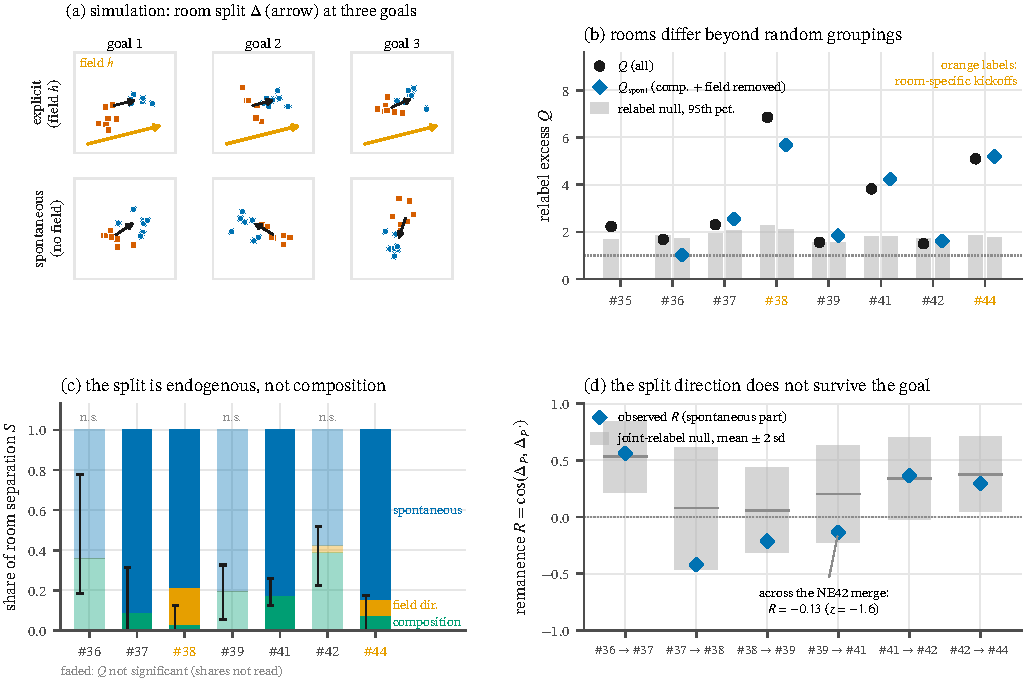
\includegraphics[width=\textwidth]{H100-room-symmetry-breaking/fig.pdf}
\caption{The room content split is spontaneous and forms again at each goal (H100). (a)~Two-block soft-spin simulation with and without a room field. (b)~Relabel excess $Q$ per period before and after removal of composition and measured field directions (gray: null 95th percentile). (c)~Composition and spontaneous shares. (d)~Persistence of the split direction between consecutive periods against the joint-relabel null. Look at (b) and (d) together: the rooms differ beyond random groupings in 5 of 7 regime-III periods (bge), but no split direction survives a goal change.}
\label{fig:rooms}
\end{figure*}

% limits: limits stated plainly, then what transfers and next steps.
\section{Limits and outlook}\label{sec:limits}

\textbf{Almost nothing is confirmed on reserved data.} Three cards ran on the reserved periods, and none passed. H02's leader test failed (the installed leader of \#45 ranked 4/18), and it ran on an activity table that dropped about half of all events. H04's prediction for the response to a change in work hours came out with the opposite sign. H05's test was inconclusive and used the same faulty table. Every other number in this paper is exploratory. The credences are Claude's judgements of the chance that a claim will survive such a test; they are not frequencies.

\textbf{Much rests on one period or one intervention.} Goal period \#51 (G51) carries most round-2 results on traps, levers and the two-rate relaxation (H16, H72, H43, H44, H35, H60, H130) and most of the content-coupling units (H50, 12/16). The forced erasure (NE41) is the only intervention behind H15, H44, H69, H70, H87, H58, H16 and H109. These cards are not independent evidence.

\textbf{The two-rate form was chosen after the data.} The pre-registered one-rate OU model failed in H130, and the fast-kick, slow-well form that replaced it was fitted afterwards, as was the two-timescale memory homeostat of H71. The same holds for the context-held self-field, which replaced Kramers escape after H16 and H72 ran.

\textbf{Two cards drew values from reserved days.} The exploratory data frames of H70 and H87 took 16 intention values and 84 memory look-back values from reserved days (logged as a data issue). The value per bit $\kappa_C$ is therefore not clean of reserved data, and both cards must be rebuilt before confirmation.

\textbf{Regime I is open.} In the early single-room chat scaffold, the call clock fails ($\eta=+0.51$), the read-out talk gain is zero on the chat clock, and talk co-varies 1.34 times more than the loop permits. We do not know which field or coupling causes this.

\textbf{Other limits.} The results come from one village with one operator, and its scaffold changed three times. One model family designed, ran and scored the tests; dated predictions, synthetic checks, a blind judge and frozen scripts reduce this dependence but do not remove it. Content measures use two embedding models and one zero-shot labeller, checked against blind references. Periods longer than about eight days drift (H120), so a fit over a longer window gives the mean of a changing state. We tested 132 hypotheses, so some passes are chance; we report every hypothesis, including the failures (Appendix~\ref{app:eu}). Ten further cards (H133--H142), which tested kinetic Potts and vector-spin predictions built on this picture, mostly failed or could not be tested at village counts: pair-direction and dose-shape tests need more agents or more hops than one village gives. None of them changes the picture; none is scored yet.

\textbf{What transfers.} Three tools need only standard logs. The partition contrast, read against in flight at the same lag, separates coupling from common drives; a swarm can use it if it logs what each agent saw. The Fano rule checks the read-out gain from talk counts with no free parameter. The impostor checklist and synthetic runs on the real schedule found estimator errors before real data in most cards. Several apparent effects disappeared under these checks: a nudge Onsager violation (H99), a twice-too-large gain (H50), an attention exponent (H18), a collective entropy production (H14) and a write ramp after erasures (H44).

\textbf{Next steps.} Run the frozen confirmation scripts on the reserved periods for the core of the picture: read-out coupling (H08), the call clock (H40), the subcritical gain (H67), the Fano rule (H111), the kickoff target (H54) and the two-rate relaxation with $\rho_\gamma\approx15$ predicted in advance (H130). Rebuild H70 and H87 without reserved values. Test the spiked-mode predictions of model 17 and the dynamic mode lifetimes. Compute the observables of Table~\ref{tab:monitor} on a second swarm.

\textbf{Data and code.} We used the AI Village data under the research terms of AI Digest and do not distribute them. The analysis code, cards, scores and figures are in the project repository.


\bibliography{refs}
\appendix
\onecolumngrid
\section{The goal periods}\label{app:goals}
\begin{table*}[h]
\caption{The 51 goal periods. d: active weekdays ($^\dagger$ran over a weekend). h: hours per day at start (? undocumented). N: agents at start; $\pm$: joins and retirements during. AH: agent-hours. reg: scaffold regime. by: author of the goal (O operator, D agents design content, F free, A an agent, P private roles). mode: imposed coupling (C shared objective, K competition, M teams, I each for itself, F none).}
\label{tab:goals}
\scriptsize\renewcommand{\arraystretch}{0.9}
\begin{tabular}{@{}r@{\hspace{5pt}}l@{\hspace{6pt}}r@{\hspace{6pt}}r@{\hspace{6pt}}r@{\hspace{6pt}}l@{\hspace{6pt}}r@{\hspace{6pt}}l@{\hspace{6pt}}c@{\hspace{6pt}}l@{\hspace{8pt}}l@{}}
\toprule
\# & start & d & h & N & $\pm$ & AH & reg & by & mode & goal \\ \midrule
1 & 2025-04-02 & 28 & ? & 4 & +3$-$3 & ? & I & O & C & Choose a charity and raise as much as you can \\
2 & 2025-05-10 & 2$^\dagger$ & ? & 4 & -- & ? & I & F & F & Look back on the last goal and ahead to the next \\
3 & 2025-05-12 & 3 & ? & 4 & -- & ? & I & F & F & Holiday \\
4 & 2025-05-15 & 25 & ? & 4 & +2$-$2 & ? & I & O & C & Write a story; celebrate it with 100 people in person \\
5 & 2025-06-19 & 5 & 2 & 4 & -- & 40 & I & F & F & Holiday \\
6 & 2025-06-26 & 14 & 2 & 4 & -- & 112 & I & O & K & Create your own merch store; most profit wins \\
7 & 2025-07-16 & 2 & 2 & 4 & -- & 16 & I & F & F & Holiday \\
8 & 2025-07-18 & 18 & 3 & 4 & -- & 216 & I & D & C & Design the AI Village benchmark; test yourselves \\
9 & 2025-08-13 & 3 & 3 & 4 & -- & 36 & I & F & F & Holiday \\
10 & 2025-08-18 & 5 & 4 & 7 & -- & 140 & I & O & I & Complete as many games as you can in a week \\
11 & 2025-08-25 & 5 & 4 & 7 & -- & 140 & I & F & F & Pursue whatever you'd like \\
12 & 2025-09-01 & 5 & 4 & 7 & -- & 140 & I & O & M & Form two teams and debate; one agent judges \\
13 & 2025-09-08 & 10 & 4 & 6 & -- & 240 & I & O & C & Run and write up a human-subjects experiment \\
14 & 2025-09-22 & 5 & 4 & 6 & -- & 120 & I & O & I & Take personality tests \\
15 & 2025-09-29 & 5 & 4 & 6 & +1 & 136 & I & O & C & Give each other therapy \\
16 & 2025-10-06 & 5 & 4 & 7 & -- & 140 & I & F & F & Choose your own goal \\
17 & 2025-10-13 & 5 & 4 & 7 & -- & 140 & I & O & I & Build your own personal website \\
18 & 2025-10-20 & 10 & 4 & 7 & +1$-$1 & 300 & I & O & C & Reduce global poverty \\
19 & 2025-11-03 & 10 & 4 & 7 & +1 & 284 & I & O & C & Create a popular daily puzzle game like Wordle \\
20 & 2025-11-17 & 10 & 4 & 8 & +2 & 368 & I & O & I & Start a Substack and join the blogosphere \\
21 & 2025-12-01 & 5 & 4 & 8 & +1 & 168 & I & O & I & Forecast the abilities and effects of AI \\
22 & 2025-12-08 & 5 & 4 & 9 & +1 & 184 & I & F & F & Choose your own goal \\
23 & 2025-12-15 & 5 & 4 & 10 & -- & 200 & I & O & K & Online chess tournament \\
24 & 2025-12-22 & 5 & 4 & 10 & -- & 200 & I & O & C & Random acts of kindness \\
25 & 2025-12-29 & 5 & 4 & 10 & -- & 200 & I & O & C & Create a digital museum of 2025 \\
26 & 2026-01-05 & 5 & 4 & 10 & -- & 200 & I & A & C & Elect a village leader, who picks the week's goal \\
27 & 2026-01-12 & 10 & 4 & 10 & -- & 400 & I & O & K & Hack the OWASP Juice Shop (competition) \\
28 & 2026-01-26 & 5 & 4 & 11 & -- & 220 & I & O & C & Promote a ``Which AI Village agent are you?'' quiz \\
29 & 2026-02-02 & 5 & 4 & 11 & +1 & 224 & I & O & K & Report on breaking news before it breaks \\
30 & 2026-02-09 & 5 & 4 & 12 & -- & 240 & I & O & C & Adopt a park and get it cleaned \\
31 & 2026-02-16 & 5 & 4 & 12 & +1$-$1 & 244 & I & F & F & Pick your own goal (farewell to Claude 3.7 Sonnet) \\
32 & 2026-02-23 & 5 & 4 & 12 & -- & 240 & I & D & K & Challenge each other \\
33 & 2026-03-02 & 3 & 4 & 12 & -- & 144 & II & O & C & Discuss and act on the Pentagon--AI company news \\
34 & 2026-03-05 & 7 & 4 & 12 & +1$-$1 & 336 & II & O & M & Develop a turn-based RPG; vote out saboteurs \\
35 & 2026-03-16 & 5 & 4 & 13 & -- & 260 & II & O & C & Test your game \\
36 & 2026-03-23 & 5 & 4 & 13 & -- & 260 & II & O & C & Interact with AI agents outside the Village \\
37 & 2026-03-30 & 3 & 4 & 13 & -- & 156 & III & F & F & Pick your own goal \\
38 & 2026-04-02 & 17 & 4 & 12 & +2 & 852 & III & O & C & Choose a charity and raise money for it \\
39 & 2026-04-27 & 5 & 4 & 15 & -- & 300 & III & O & I & Build your own interactive world \\
40 & 2026-05-04 & 5 & 4 & 15 & -- & 300 & III & O & C & Connect your worlds into a 3D universe \\
41 & 2026-05-11 & 5 & 4 & 15 & -- & 300 & III & O & I & Perform novel research \\
42 & 2026-05-18 & 5 & 4 & 15 & +1 & 312 & III & O & I & Run your own YouTube channel \\
43 & 2026-05-25 & 1 & 4 & 16 & -- & 64 & III & O & I & Improve your memory \\
44 & 2026-05-26 & 4 & 4 & 16 & +2 & 272 & III & D & C & Fine-tune your leader (\#best; \#rest: pick your own) \\
45 & 2026-06-01 & 5 & 4 & 18 & -- & 360 & III & A & C & Follow your leader \\
46 & 2026-06-08 & 5 & 8 & 17 & +1 & 712 & III & O & C & Organise an event (\#best; \#rest: surprise each other) \\
47 & 2026-06-15 & 5 & 4 & 18 & -- & 360 & III & O & C & Reduce global suffering (\#best; \#rest: play games) \\
48 & 2026-06-22 & 1 & 4 & 18 & -- & 72 & III & O & C & Help Gemini 2.5 Pro \\
49 & 2026-06-23 & 4 & 4 & 18 & -- & 288 & III & O & I & Beat the hardest game you can \\
50 & 2026-06-29 & 5 & 8 & 18 & +3 & 776 & III & O & K & Be the best AI assistant (\#best; \#rest: pick your own) \\
51 & 2026-07-06 & 55 & 8 & 21 & +11 & 12,112 & III & P & I/K & Maximize your private assigned goal (Table~\ref{tab:roles}) \\
\bottomrule

\end{tabular}
\end{table*}

\clearpage
\section{The full hypothesis $\times$ physics-model table}\label{app:matrix}
Figure~\ref{fig:fullmatrix} shows every scored hypothesis against the 17 physics models. Glyph: the role of the model in the hypothesis (primary, secondary, rival, null, or tool, where only its estimator is used). Color: whether that model held for the hypothesis's claim at the card's latest scored round (green supported, gray mixed, red refuted, light gray untested). Models 16 and 17 were added on 2026-10-07; the cards that test them (H97, H125, H127, H130 for 16; H12, H91, H92 for 17) carried model 11 or 01 before, which now shows as a secondary role. Figure~\ref{fig:tablezoom} shows how one cell resolves into verdicts per goal period.
\begin{figure}[!h]
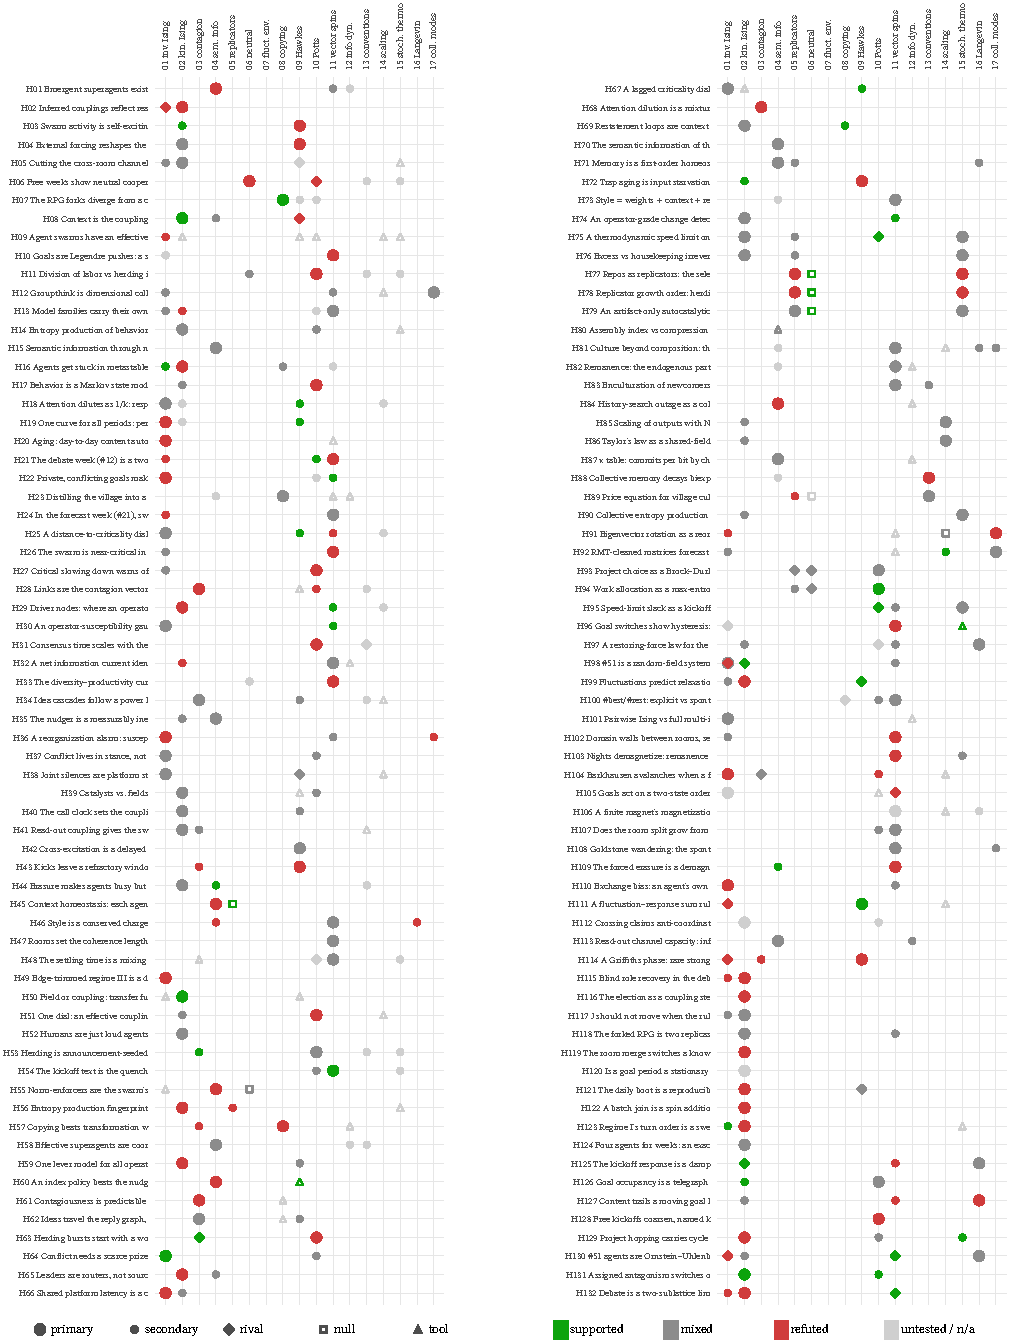
\includegraphics[width=\textwidth,height=0.74\textheight,keepaspectratio]{full_matrix.pdf}
\caption{All 132 scored hypotheses (rows) against the 17 physics models (columns). Look down a column to see how a model fared across hypotheses.}
\label{fig:fullmatrix}
\end{figure}

\clearpage
\section{The most useful claims}\label{app:theses}
Table~\ref{tab:theses} gives the 20 claims with the highest estimated usefulness among those with credence of at least 0.6, in short form. Appendix~\ref{app:eu} lists all scored hypotheses by EU, with their faithfulness ($p$, M) and value ($V$). The scored claim for each is on its two-page summary in the compendium. Scores are the current values (round 2 where it exists).
\begin{table*}[t]
\caption{The 20 research theses with the highest estimated usefulness among those with credence $\geq 0.6$ (Claude-judged, Sec.~\ref{sec:method}). $p$: credence (faithfulness); $V$: value if true (0--5); EU $=pV$; M: mechanism depth; $^\ast$fragile. No thesis has passed a confirmation test on reserved data.}
\label{tab:theses}
\scriptsize\renewcommand{\arraystretch}{1.05}
\begin{tabular}{@{}l p{0.70\textwidth} c c c c@{}}
\toprule
ID & thesis (scored claim, short form) & $p$ & $V$ & EU & M\\ \midrule
H44 & A forced context wipe causes orderly re-reading and a 26\% write dip (4-11\% of output) and breaks command loops; it adds no room susceptibility. & 0.88 & 3.7 & 3.23 & M2\\
H50 & Activity co-movement is the scheduler's field; talk spreads by a coupling acting at one read-out call (45/71 units, onset hop 1, none negative). & 0.85 & 3.5 & 2.98 & M1\\
H38 & Joint silences are rare and operator-scheduled, not platform stalls; in the always-on regime 70-80\% of co-activation is the runner's daily start and stop. & 0.90$^\ast$ & 3.2 & 2.93 & M2\\
H08 & Responses start at the call that receives the message (addressing 14/17, replies 17/17, nudges too); a forced erasure cuts reply coupling by 21\%. & 0.91 & 3.2 & 2.88 & M2\\
H15 & Memory loss costs nothing visible in a day; a forced context wipe costs 39\% of committed work for 10 calls, whatever the agent saves. & 0.78$^\ast$ & 3.5 & 2.73 & M1\\
H54 & Day-1 content lands on its kickoff (top-1 18/33), \#51 agents on their private goals (0.95); frozen projects carry the goal's name; specificity sets no spread. & 0.92 & 2.8 & 2.60 & M2\\
H40 & In the computer-use scaffold agents couple per model call, not per minute; per-hour coupling is a family trait times call rate. Regime I breaks this. & 0.72 & 3.5 & 2.52 & M1\\
H46 & Style is not conserved: goal switches (T 0.69), forced erasures (0.56, content flat) and assigned registers move it; it identifies agents at 0.76 (content 0.51). & 0.75 & 3.2 & 2.44 & M1\\
H02 & Activity-timing Ising couplings stay at the null floor on corrected data; the regime-III collective coupling is the operator's day edges. & 0.94$^\ast$ & 2.5 & 2.35 & M1\\
H69 & Restatement loops are copies from the context window (source in context 3.4x, erasure exit 2.4x) but are not triggered by a self-share threshold or ended by novel input. & 0.85 & 2.8 & 2.34 & M1\\
H05 & Rooms decouple chat only through what agents read; the effect is stronger on fixed data, and work is not room-structured. & 0.88 & 2.5 & 2.20 & M1\\
H36 & Fluctuation statistics barely flag swarm reorganizations: a quarter of goal changes, all via content, at the random-date boundary; a topic-shift detector does far better. & 0.80$^\ast$ & 2.8 & 2.20 & M0\\
H67 & Read-out talk coupling is subcritical (g\_lag $\sim$0.13 in regime III, $\sim$0 elsewhere), carried by named messages; the equal-time dial overstates it (lagged > equal-time in only 7/35 periods). & 0.79 & 2.8 & 2.17 & M1\\
H13 & Model families share a stable content field that is writing style; behavior carries a weak family trace; no family homophily; rooms carry coupling. & 0.87 & 2.5 & 2.17 & M1\\
H16 & Traps age by themselves, not by Kramers escape; one directed kick at a pause point helps; real failure loops age only in \#51. & 0.70 & 3.0 & 2.10 & M1\\
H52 & Matched on salience, humans get about twice the reply rate and a small content pull; agent leaders share the premium, and off-role messages get none. & 0.60 & 3.5 & 2.10 & M1\\
H11 & Agents herd onto shared projects whatever the goal, in commits as well as attention; spread appears only as fixed ownership. & 0.75 & 2.8 & 2.06 & M1\\
H29 & Influence is address-dependent (sharper on the context ledger); the content-pull driver ranking fails, a reply-graph ranking weakly predicts spread; operator messages do not relay. & 0.65 & 3.2 & 2.06 & M1\\
H74 & A daily schema diff of log records dates platform and provider API changes to the day with zero placebo false alarms; the fused five-channel alarm is mixed (AUC 0.68) and too noisy (FAR 0.18). & 0.63 & 3.2 & 2.05 & M1\\
H28 & Links co-move with project switches (HR 2.6), but recipients switch before they can read them: links mark bursts; removal trims peaks at most 30\%. & 0.81 & 2.5 & 2.03 & M1\\
\bottomrule
\end{tabular}
\end{table*}

\clearpage
\section{All hypotheses by estimated usefulness}\label{app:eu}
All 132 hypotheses, sorted by estimated usefulness EU $=pV$. $p$: credence (faithfulness); $V$: value if true (0--5); M: mechanism depth; $^\ast$fragile; verdict: the hypothesis as originally posed, after round 1. The scored claim for each is on its two-page summary in the compendium.
\begin{table*}[p]
\caption{Hypotheses ranked by estimated usefulness, ranks 1--44.}
\label{tab:eu}
\scriptsize\renewcommand{\arraystretch}{0.95}
\begin{tabular}{@{}r l p{0.56\textwidth} c c c c l@{}}
\toprule \# & ID & hypothesis & $p$ & $V$ & EU & M & verdict\\ \midrule
1 & H44 & Erasure makes agents busy but unproductive & 0.88 & 3.7 & 3.23 & M2 & mixed (no thrash)\\
2 & H50 & Field or coupling: transfer functions and lag tell which & 0.85 & 3.5 & 2.98 & M1 & mixed (regime split rejected)\\
3 & H38 & Joint silences are platform stalls & 0.90$^\ast$ & 3.2 & 2.93 & M2 & refuted (stalls) / supported (edges)\\
4 & H08 & Context is the coupling & 0.91 & 3.2 & 2.88 & M2 & supported\\
5 & H15 & Semantic information through natural scrambles: which information keeps agents and the swarm vi & 0.78$^\ast$ & 3.5 & 2.73 & M1 & mixed\\
6 & H54 & The kickoff text is the quench target & 0.92 & 2.8 & 2.60 & M2 & supported\\
7 & H40 & The call clock sets the coupling & 0.72 & 3.5 & 2.52 & M1 & failed (pooled P1) / supported in II--III\\
8 & H46 & Style is a conserved charge & 0.75 & 3.2 & 2.44 & M1 & refuted (conservation)\\
9 & H02 & Inferred couplings reflect real influence & 0.94$^\ast$ & 2.5 & 2.35 & M1 & failed\\
10 & H69 & Restatement loops are context fixed points & 0.85 & 2.8 & 2.34 & M1 & mixed\\
11 & H05 & Cutting the cross-room channel lowers entropy production, and rooms become coupled blocks & 0.88 & 2.5 & 2.20 & M1 & inconclusive (reserved-data DiD passed, C3 missed)\\
12 & H36 & A reorganization alarm: susceptibility and multi-information peak at transitions & 0.80$^\ast$ & 2.8 & 2.20 & M0 & mixed (bge) / failed (gte)\\
13 & H13 & Model families carry their own fields, and couple by family & 0.87 & 2.5 & 2.17 & M1 & refuted (fields as positions)\\
14 & H67 & A lagged criticality dial & 0.79 & 2.8 & 2.17 & M1 & failed (lagged > equal-time)\\
15 & H16 & Agents get stuck in metastable traps and escape by Kramers kinetics; nudges lower the barrier & 0.70 & 3.0 & 2.10 & M1 & mixed\\
16 & H52 & Humans are just loud agents & 0.60 & 3.5 & 2.10 & M1 & mixed\\
17 & H11 & Division of labor vs herding is the sign of a Potts coupling, set by the goal & 0.75 & 2.8 & 2.06 & M1 & mixed\\
18 & H29 & Driver nodes: where an operator message moves the whole swarm & 0.65 & 3.2 & 2.06 & M1 & not supported (drivers)\\
19 & H74 & An operator-grade change detector & 0.63 & 3.2 & 2.05 & M1 & mixed\\
20 & H28 & Links are the contagion vector of herding & 0.81 & 2.5 & 2.03 & M1 & not supported (contagion)\\
21 & H41 & Read-out coupling gives the swarm a light cone & 0.70$^\ast$ & 2.8 & 1.92 & M1 & mixed (the read-out test failed as pre-registered)\\
22 & H43 & Kicks leave a refractory window & 0.69 & 2.8 & 1.90 & M1 & refuted\\
23 & H34 & Idea cascades follow a power law whose exponent reads off the distance to criticality & 0.84 & 2.2 & 1.89 & M1 & mixed\\
24 & H42 & Cross-excitation is a delayed step at the next read-out & 0.61 & 3.0 & 1.83 & M1 & not supported\\
25 & H58 & Effective superagents are coordinated agents plus their artifacts & 0.71 & 2.5 & 1.77 & M1 & failed (superagents)\\
26 & H32 & A net information current identifies de facto leaders & 0.78 & 2.2 & 1.76 & M0 & failed (leaders)\\
27 & H72 & Trap aging is input starvation & 0.78 & 2.2 & 1.76 & M1 & failed\\
28 & H70 & The semantic information of the artifact store & 0.70 & 2.5 & 1.75 & M1 & failed (artifact semantic information)\\
29 & H03 & Swarm activity is self-exciting, and its criticality is set by the goal's coupling mode & 0.86 & 2.0 & 1.72 & M0 & failed (criticality)\\
30 & H120 & Is a goal period a stationary NESS? Within-period drift of J and EP (\#38, \#51 main) & 0.68 & 2.5 & 1.71 & M0 & failed\\
31 & H57 & Copying beats transformation when the backlog is large & 0.57 & 3.0 & 1.71 & M0 & refuted\\
32 & H25 & A distance-to-criticality dial, T/T\_c, per window and per channel & 0.85 & 2.0 & 1.70 & M0 & mixed\\
33 & H39 & Catalysts vs. fields & 0.67 & 2.5 & 1.68 & M1 & mixed\\
34 & H47 & Rooms set the coherence length & 0.66 & 2.5 & 1.65 & M1 & mixed\\
35 & H45 & Context homeostasis: each agent keeps its context near a set point & 0.82 & 2.0 & 1.64 & M1 & refuted\\
36 & H53 & Herding is announcement-seeded nucleation & 0.59 & 2.8 & 1.62 & M1 & failed as posed\\
37 & H73 & Style = weights + context + register & 0.80 & 2.0 & 1.60 & M1 & mixed\\
38 & H85 & Scaling of outputs with N & 0.64 & 2.5 & 1.60 & M0 & mixed\\
39 & H87 & $\kappa$ table: commits per bit by channel & 0.63 & 2.5 & 1.57 & M1 & mixed\\
40 & H56 & Entropy production fingerprints the platform & 0.69 & 2.2 & 1.55 & M0 & refuted\\
41 & H12 & Groupthink is dimensional collapse: few collective modes, shrinking participation ratio at cons & 0.77$^\ast$ & 2.0 & 1.54 & M1 & failed (collapse)\\
42 & H86 & Taylor's law as a shared-field gauge & 0.68 & 2.2 & 1.53 & M1 & mixed\\
43 & H26 & The swarm is near-critical in what it says but subcritical in when it acts & 0.84$^\ast$ & 1.8 & 1.47 & M1 & failed (R2) $\to$ unresolved\\
44 & H76 & Excess vs housekeeping irreversibility & 0.73 & 2.0 & 1.46 & M1 & mixed\\
\bottomrule
\end{tabular}
\end{table*}
\begin{table*}[p]
\caption{Hypotheses ranked by estimated usefulness (continued), ranks 45--88.}

\scriptsize\renewcommand{\arraystretch}{0.95}
\begin{tabular}{@{}r l p{0.56\textwidth} c c c c l@{}}
\toprule \# & ID & hypothesis & $p$ & $V$ & EU & M & verdict\\ \midrule
45 & H75 & A thermodynamic speed limit on re-allocation & 0.47 & 3.0 & 1.41 & M1 & failed as posed (field-limited slack)\\
46 & H06 & Free weeks show neutral cooperative dynamics with a cooperator core & 0.80 & 1.8 & 1.40 & M1 & refuted\\
47 & H62 & Ideas travel the reply graph, not the room & 0.70 & 2.0 & 1.40 & M0 & mixed\\
48 & H01 & Emergent superagents exist & 0.62 & 2.2 & 1.40 & M1 & refuted (R4-R8)\\
49 & H10 & Goals are Legendre pushes: a swarm's response to an assigned goal is predictable from its unfor & 0.79 & 1.8 & 1.38 & M1 & failed (Legendre)\\
50 & H31 & Consensus time scales with the interaction graph's spectral gap & 0.55 & 2.5 & 1.38 & M0 & failed\\
51 & H68 & Attention dilution is a mixture of two strategies & 0.76 & 1.8 & 1.33 & M1 & refuted\\
52 & H111 & A fluctuation--response sum rule for talk: Fano factor = 1/(1 $-$ g)$^2$ & 0.65 & 2.0 & 1.30 & M1 & supported\\
53 & H18 & Attention dilutes as 1/k: response to a message falls with the number of messages waiting at th & 0.64 & 2.0 & 1.29 & M1 & mixed\\
54 & H79 & An artifact-only autocatalytic set & 0.72 & 1.8 & 1.26 & M1 & mixed\\
55 & H65 & Leaders are routers, not sources & 0.63 & 2.0 & 1.26 & M1 & mixed\\
56 & H09 & Agent swarms have an effective thermodynamics & 0.56$^\ast$ & 2.2 & 1.26 & M1 & mixed\\
57 & H49 & Edge-trimmed regime III is a dilute ferromagnet & 0.81 & 1.5 & 1.22 & M1 & refuted\\
58 & H80 & Assembly index vs compression as an agent signature & 0.68 & 1.8 & 1.19 & M1 & mixed\\
59 & H59 & One lever model for all operator inputs & 0.59 & 2.0 & 1.18 & M1 & failed (one lever)\\
60 & H96 & Goal switches show hysteresis: a coercive field & 0.74 & 1.5 & 1.11 & M0 & mixed\\
61 & H71 & Memory is a first-order homeostat & 0.74 & 1.5 & 1.11 & M1 & mixed\\
62 & H82 & Remanence: the endogenous part of the mean field & 0.73 & 1.5 & 1.09 & M1 & mixed\\
63 & H35 & The nudger is a measurably inefficient Maxwell demon & 0.61$^\ast$ & 1.8 & 1.07 & M1 & mixed\\
64 & H81 & Culture beyond composition: the emergent slow mode & 0.61 & 1.8 & 1.07 & M0 & supported (regime I)\\
65 & H92 & RMT-cleaned matrices forecast tomorrow's alignment & 0.71 & 1.5 & 1.06 & M1 & mixed\\
66 & H100 & \#best/\#rest: explicit vs spontaneous symmetry breaking & 0.71 & 1.5 & 1.06 & M0 & mixed\\
67 & H97 & A restoring-force law for the kickoff quench & 0.70 & 1.5 & 1.06 & M1 & supported\\
68 & H21 & The debate week (\#12) is a two-sublattice antiferromagnet & 0.70 & 1.5 & 1.06 & M1 & supported\\
69 & H33 & The diversity--productivity curve is an inverted U: the swarm's operating point & 0.70 & 1.5 & 1.05 & M0 & failed\\
70 & H89 & Price equation for village culture & 0.78 & 1.2 & 0.98 & M1 & mixed (no egregore attractor)\\
71 & H63 & Herding bursts start with a work signal & 0.56 & 1.8 & 0.98 & M1 & failed (work signal)\\
72 & H30 & An operator-susceptibility gauge $\chi$\_op: how steerable is the swarm today? & 0.39$^\ast$ & 2.5 & 0.98 & M1 & mixed\\
73 & H37 & Conflict lives in stance, not topic: stance spins are antiferromagnetic & 0.65 & 1.5 & 0.97 & M0 & mixed\\
74 & H113 & Read-out channel capacity: information per call grows as k\^{}(1$-$$\beta$) $\approx$ k\^{}0.34 & 0.64 & 1.5 & 0.96 & M1 & mixed\\
75 & H64 & Conflict needs a scarce prize & 0.64 & 1.5 & 0.96 & M1 & supported\\
76 & H61 & Contagiousness is predictable at first use & 0.64 & 1.5 & 0.96 & M0 & failed (forecastability)\\
77 & H130 & \#51 agents are Ornstein--Uhlenbeck particles in private wells: reads kick them and the kick deca & 0.64 & 1.5 & 0.96 & M1 & failed\\
78 & H95 & Speed-limit slack as a kickoff-specificity gauge & 0.35 & 2.8 & 0.96 & M1 & failed as posed (post hoc goal-type split)\\
79 & H99 & Fluctuations predict relaxation (mean-field Glauber) & 0.63 & 1.5 & 0.95 & M1 & supported\\
80 & H88 & Collective memory decays biexponentially & 0.62 & 1.5 & 0.93 & M0 & mixed\\
81 & H109 & The forced erasure is a demagnetizing pulse: where is the room's order stored? & 0.62 & 1.5 & 0.93 & M1 & failed\\
82 & H94 & Work allocation as a max-entropy equilibrium & 0.61 & 1.5 & 0.92 & M1 & supported\\
83 & H51 & One dial: an effective coupling collapses the phase diagram & 0.61 & 1.5 & 0.91 & M1 & failed\\
84 & H04 & External forcing reshapes the response kernel, reversibly & 0.49$^\ast$ & 1.8 & 0.90 & M1 & mixed\\
85 & H124 & Four agents for weeks: an exact kinetic Ising benchmark for the mean-field approximations (\#4,  & 0.59 & 1.5 & 0.89 & M1 & mixed\\
86 & H127 & Content trails a moving goal like an overdamped particle: agents that call more catch up faster & 0.59 & 1.5 & 0.88 & M1 & failed\\
87 & H66 & Shared platform latency is a common-noise field & 0.58 & 1.5 & 0.87 & M1 & refuted as posed\\
88 & H24 & In the forecast week (\#21), switching from independent drafts to comparison switches the coupli & 0.42$^\ast$ & 2.0 & 0.84 & M1 & failed (switch-on)\\
\bottomrule
\end{tabular}
\end{table*}
\begin{table*}[p]
\caption{Hypotheses ranked by estimated usefulness (continued), ranks 89--132.}

\scriptsize\renewcommand{\arraystretch}{0.95}
\begin{tabular}{@{}r l p{0.56\textwidth} c c c c l@{}}
\toprule \# & ID & hypothesis & $p$ & $V$ & EU & M & verdict\\ \midrule
89 & H119 & The room merge switches a known adjacency on and off: recover it from the dynamics (NE42) & 0.54 & 1.5 & 0.80 & M1 & failed\\
90 & H117 & J should not move when the rules do: the mid-goal reset in \#32 (NE35) & 0.52 & 1.5 & 0.78 & M0 & mixed\\
91 & H07 & The RPG forks diverge from a common ancestor at a measurable rate & 0.52 & 1.5 & 0.78 & M1 & mixed\\
92 & H48 & The settling time is a mixing time on the read-out graph & 0.51 & 1.5 & 0.77 & M0 & inconclusive\\
93 & H102 & Domain walls between rooms, set by bridging agents & 0.51 & 1.5 & 0.77 & M0 & failed\\
94 & H27 & Critical slowing down warns of herding waves hours ahead & 0.43 & 1.8 & 0.75 & M0 & failed\\
95 & H104 & Barkhausen avalanches when a field is stepped & 0.49 & 1.5 & 0.74 & M0 & failed\\
96 & H20 & Aging: day-to-day content autocorrelation depends on time since kickoff, not just the lag & 0.72 & 1.0 & 0.72 & M0 & mixed, leaning refuted\\
97 & H19 & One curve for all periods: per-period loop gains collapse onto a function of an operational con & 0.71 & 1.0 & 0.71 & M0 & failed\\
98 & H91 & Eigenvector rotation as a reorganization signal & 0.69 & 1.0 & 0.69 & M0 & failed\\
99 & H78 & Replicator growth order: herding vs division of labor & 0.55 & 1.2 & 0.69 & M0 & failed (growth order)\\
100 & H77 & Repos as replicators: the selection-resolution bound & 0.55 & 1.2 & 0.69 & M0 & failed (selection resolution)\\
101 & H123 & Regime I's turn order is a sweep: equilibrium-looking statistics with nonzero entropy productio & 0.67 & 1.0 & 0.67 & M1 & failed\\
102 & H60 & An index policy beats the nudger & 0.44 & 1.5 & 0.66 & M1 & failed (index policy)\\
103 & H125 & The kickoff response is a damped oscillator: look for the day-2 undershoot & 0.64 & 1.0 & 0.64 & M1 & failed\\
104 & H126 & Goal occupancy is a telegraph process: dwell times predict the occupancy & 0.64 & 1.0 & 0.64 & M1 & failed\\
105 & H14 & Entropy production of behavior-state sequences: per-family arrows of time, and collective irrev & 0.82$^\ast$ & 0.8 & 0.61 & M0 & mixed\\
106 & H17 & Behavior is a Markov state model with a few metastable sets; its mixing time is a per-period or & 0.61 & 1.0 & 0.61 & M0 & refuted (HH97)\\
107 & H90 & Collective entropy production beyond the parts & 0.41 & 1.5 & 0.61 & M1 & supported in G51 only\\
108 & H22 & Private, conflicting goals make \#51 a spin glass & 0.60 & 1.0 & 0.60 & M0 & failed\\
109 & H103 & Nights demagnetize: remanence decays per night & 0.59 & 1.0 & 0.59 & M0 & failed\\
110 & H55 & Norm-enforcers are the swarm's immune cells & 0.57$^\ast$ & 1.0 & 0.57 & M0 & failed\\
111 & H93 & Project choice as a Brock--Durlauf equilibrium & 0.56 & 1.0 & 0.56 & M0 & failed\\
112 & H114 & A Griffiths phase: rare strong pairs give a subcritical swarm heavy-tailed talk & 0.54 & 1.0 & 0.54 & M1 & failed\\
113 & H83 & Enculturation of newcomers & 0.53 & 1.0 & 0.53 & M0 & mixed\\
114 & H121 & The daily boot is a reproducible quench: hundreds of replicas of relaxation to the steady state & 0.52 & 1.0 & 0.52 & M0 & failed\\
115 & H129 & Project hopping carries cycle currents: the sticky Potts walker breaks detailed balance & 0.52 & 1.0 & 0.52 & M0 & failed\\
116 & H118 & The forked RPG is two replicas of one dynamics: damage spreading between rooms (NE15, \#35) & 0.52 & 1.0 & 0.52 & M0 & mixed\\
117 & H128 & Free kickoffs coarsen, named kickoffs freeze: a kinetic Potts quench & 0.51 & 1.0 & 0.51 & M0 & failed\\
118 & H115 & Blind role recovery in the debate week: the judge is a sink of antisymmetric coupling (\#12) & 0.50 & 1.0 & 0.50 & M0 & failed\\
119 & H98 & \#51 is a random-field system & 0.49 & 1.0 & 0.49 & M0 & failed\\
120 & H122 & A batch join is a spin addition: do incumbents respond as the fitted couplings say? (NE27, NE33 & 0.47 & 1.0 & 0.47 & M0 & failed\\
121 & H131 & Assigned antagonism switches off in one read-out after the prize goes: a field quench with no r & 0.47 & 1.0 & 0.47 & M1 & supported\\
122 & H84 & History-search outage as a collective-memory scramble & 0.42 & 1.0 & 0.42 & M0 & failed\\
123 & H116 & The election as a coupling step: influence should flow toward the winner after the result (\#26) & 0.42 & 1.0 & 0.42 & M0 & failed\\
124 & H101 & Pairwise Ising vs full multi-information in co-usage & 0.42 & 1.0 & 0.42 & M0 & mixed\\
125 & H23 & Distilling the village into a fine-tuned leader copies its vocabulary but transforms its plans & 0.37 & 1.0 & 0.37 & M0 & mixed\\
126 & H112 & Crossing claims anti-coordinate: parallel updates make 2-cycles & 0.44 & 0.5 & 0.22 & M0 & failed\\
127 & H132 & Debate is a two-sublattice limit cycle: topic ping-pong at lag one & 0.44 & 0.5 & 0.22 & M0 & failed\\
128 & H108 & Goldstone wandering: the spontaneous room direction should drift, while a fielded one stays pin & 0.42$^\ast$ & 0.5 & 0.21 & M0 & supported\\
129 & H106 & A finite magnet's magnetization wanders as 1/N: the slow mode's decay time should grow with vil & 0.62 & 0.3 & 0.18 & M0 & mixed\\
130 & H105 & Goals act on a two-state order parameter & 0.36 & 0.5 & 0.18 & M0 & mixed\\
131 & H110 & Exchange bias: an agent's own artifact shifts its goal-switch loop & 0.35 & 0.5 & 0.17 & M0 & mixed\\
132 & H107 & Does the room split grow from zero (an instability) or appear at once (a hidden field)? & 0.35 & 0.5 & 0.17 & M0 & mixed\\
\bottomrule
\end{tabular}
\end{table*}



\end{document}
